\documentclass[thesis]{thesis-gwu}[2020/02/03]

% =============================================================================
% --- 1. CORE & FONT SETUP (Robustness First)
% =============================================================================
\usepackage[T1]{fontenc}      % Use modern font encoding for better character and hyphenation support
\usepackage{setspace}         % For controlling line spacing (e.g., in appendix)
\usepackage{amsmath}          % Essential for advanced mathematics typesetting


% =============================================================================
% --- 2. GRAPHICS, FIGURES, & TIKZ
% =============================================================================
\usepackage{graphicx}         % For including images with \includegraphics
\usepackage{float}            % Improved control over float placement (e.g., [H])
\usepackage{pgfplots}         % For creating plots and charts
\pgfplotsset{compat=1.18}
\usepackage{tikz}             % For drawing vector graphics
\usetikzlibrary{shapes, arrows, calc, positioning, shadows, fit, backgrounds}


% Optional: TikZ externalization to speed up compile times.
% Keep this commented out until you have many complex figures.
% \usepgfplotslibrary{external}
% \tikzexternalize
% \tikzsetexternalprefix{cache/}


% =============================================================================
% --- 3. TABLES & FORMATTING
% =============================================================================
\usepackage{booktabs}         % For professional-quality table rules (\toprule, \midrule, \bottomrule)
\usepackage{longtable}        % For tables that span multiple pages
\usepackage{tabularx}         % For tables with columns that automatically adjust width
\usepackage{array}            % For defining custom column types
\usepackage{multirow}         % For creating table cells that span multiple rows
\usepackage{makecell}         % For line breaks and advanced formatting within cells
\usepackage{colortbl}         % For adding color to table cells, rows, or columns
\usepackage{adjustbox}        % For scaling/resizing content (use with caution on tables)

% Custom column types for tables
\newcolumntype{L}[1]{>{\raggedright\arraybackslash}p{#1}}
\newcolumntype{Y}{>{\centering\arraybackslash}X} % Relies on tabularx


% =============================================================================
% --- 4. CAPTIONS & LISTINGS
% =============================================================================
\usepackage{caption}          % For customizing captions of floats
\captionsetup{
    justification=justified,  % Justify multi-line captions
    singlelinecheck=false,    % Apply justification even to single-line captions
    font=it                   % Italicize caption text
}

\usepackage{listings}         % For typesetting source code
\renewcommand{\lstlistingname}{Source Code}
\renewcommand{\lstlistlistingname}{List of Source Code} % Fix for the list name
\definecolor{codegreen}{rgb}{0,0.6,0}
\definecolor{codegray}{rgb}{0.5,0.5,0.5}
\definecolor{codepurple}{rgb}{0.58,0,0.82}
\definecolor{backcolour}{rgb}{0.95,0.95,0.92}
\lstset{
    language=Python,
    backgroundcolor=\color{backcolour},
    commentstyle=\color{codegreen},
    keywordstyle=\color{magenta},
    numberstyle=\tiny\color{codegray},
    stringstyle=\color{codepurple},
    basicstyle=\fontsize{8}{9}\selectfont\ttfamily,
    breaklines=true,
    captionpos=b,
    keepspaces=true,
    numbers=left,
    numbersep=5pt,
    showstringspaces=false,
    tabsize=2,
    frame=single,
    rulecolor=\color{black},
    title=\lstname
}
% --- Color Definitions ---
\definecolor{backgroundColour}{gray}{0.96}  % A very light gray for the background

% --- Custom Style for Prompts ---
\lstdefinestyle{promptstyle}{
    language={[plain]tex}, % Treat as plain text
    basicstyle=\ttfamily\small,
    breaklines=true,
    captionpos=b,
    frame=single,
    rulecolor=\color{black!30},
    backgroundcolor=\color{backgroundColour},
    keepspaces=true,
    showspaces=false,
    showstringspaces=false,
    tabsize=2,
    % Highlight the placeholders like {chunk}
    moredelim=**[is][\color{red}\bfseries]{@}{@},
}
% --- Color Definitions ---
\definecolor{commentGreen}{HTML}{228B22}
\definecolor{stringRed}{HTML}{D22D2D}
\definecolor{keywordBlue}{HTML}{0000FF}
\definecolor{jsonBoolean}{HTML}{F0AD4E}
\definecolor{backgroundColour}{gray}{0.96}

% --- 1. Define the JSON language from scratch ---
% This creates a new language called 'JSON' that listings will understand.
\lstdefinelanguage{JSON}{
    keywords={true, false, null},
    keywordstyle=\color{jsonBoolean}\bfseries,
    string=[s]{"}{"}, % Defines strings as anything between double quotes
    stringstyle=\color{stringRed},
    comment=[l]{//},   % Allows for line comments (like in JSONC)
    commentstyle=\color{commentGreen},
    morecomment=[s]{/*}{*/}, % Allows for block comments
    ndkeywords={0,1,2,3,4,5,6,7,8,9} % Ensures numbers are not treated as keywords
}

% --- 2. Define a style that USES our new JSON language ---
\lstdefinestyle{json}{
    language=JSON, % Use the language we just defined above
    backgroundcolor=\color{backgroundColour},
    basicstyle=\ttfamily\small,
    breaklines=true,
    captionpos=b,
    frame=single,
    keepspaces=true,
    numbers=left,
    numbersep=5pt,
    numberstyle=\tiny\color{gray},
    rulecolor=\color{black!30},
    showspaces=false,
    showstringspaces=false,
    tabsize=2,
}

% --- Custom Cypher Style Definition (no changes needed here) ---
\lstdefinestyle{cypher}{
    language=SQL,
    morekeywords={
        MATCH, WHERE, WITH, RETURN, ORDER, BY, ASC, DESC, OPTIONAL, ALL, IN, NOT,
        CREATE, DELETE, SET, REMOVE, ON, MERGE, AND, OR, XOR,
        CASE, WHEN, THEN, ELSE, END,
        DISTINCT, AS, UNION, SKIP, LIMIT,
        STARTS, ENDS, CONTAINS,
        TRUE, FALSE, NULL,
        collect, nodes, size, toFloat, toLower, id, displayName
    },
    keywordstyle=\color{keywordBlue}\bfseries,
    comment=[l]{//},
    commentstyle=\color{commentGreen}\itshape,
    stringstyle=\color{stringRed},
    basicstyle=\ttfamily\small,
    breaklines=true,
    captionpos=b,
    frame=single,
    rulecolor=\color{black!30},
    backgroundcolor=\color{backgroundColour},
    keepspaces=true,
    numbers=left,
    numbersep=5pt,
    numberstyle=\tiny\color{gray},
    showspaces=false,
    showstringspaces=false,
    tabsize=2,
}

% =============================================================================
% --- 5. BIBLIOGRAPHY & REFERENCES (biblatex)
% =============================================================================
\usepackage[style=apa, backend=biber, language=american]{biblatex}
\addbibresource{mybib.bib} % Ensure this file exists and is correct


% =============================================================================
% --- 6. GLOSSARY & ACRONYMS
% =============================================================================
%\usepackage{glossaries}       % Explicitly load the glossaries package
%\makenoidxglossaries         % Command to generate the glossaries/acronyms lists


% =============================================================================
% --- 7. UTILITY & MISC PACKAGES
% =_===========================================================================
\usepackage{comment}          % For commenting out large blocks of text
\usepackage{pdfpages}         % For inserting pages from external PDF files
\usepackage{afterpage}        % For executing commands after the current page is shipped out
%\usepackage{lipsum}           % For dummy text during development (remove for final version)


% =============================================================================
% --- 8. HYPERLINKS (MUST BE LOADED LAST)
% =============================================================================
\hypersetup{
    pdftitle={Using Large Language Models to Convert Documents to Knowledge Graphs to Check for Completeness and Consistency},
    pdfauthor={Michael Wacey},
    pdfsubject={A Brief Description of the Research Field},
    pdfkeywords={keyword1, keyword2, keyword3}
}
% Custom color for biblatex citations, needs to be defined before hyperref uses it
\definecolor{DarkGreen}{rgb}{0,0.5,0}


% =============================================================================
% --- DOCUMENT START
% =============================================================================

% Load frontmatter definitions from your template
% !TEX root = ../thesis.tex
%==============================================================================
% --- CORE THESIS INFORMATION ---
%==============================================================================
% Full title of the thesis. Capitalize all significant words.
\title{Mnemosyne: Using Large Language Models to Convert Documents to Knowledge Graphs to Check for Completeness and Consistency}

% Author's name as it should appear on the title page.
\author{Michael Wacey}

% Year of completion for copyright page and other parts of the document.
\year=2026

% The person or entity holding the copyright.
% By default, this is the author. Uncomment to change it.
%\copyrightholder{Someone Else}


%==============================================================================
% --- DEGREE & GRADUATION INFORMATION ---
%==============================================================================
% Previous Degrees
\bachelordegree{B.S.}
\bsdepartment{Computer Science}
\bsschool{Washington University in St. Louis}
\bsgrad{June 1985}

\masterdegree{M.S.}
\msdepartment{Computer Science}
\msschool{Drexel University}
\msgrad{December 1990}
\showmsdegree % Use \hidemsdegree if you do not want to display the Master's degree.

% Doctoral Degree Information
\phdschool{The School of Engineering and Applied Science}
\phdgrad{March 8, 2026}
\defensedate{December 18, 2025}


%==============================================================================
% --- COMMITTEE MEMBERS ---
%==============================================================================
% This section defines all committee members for the committee page.

% -- Praxis Director / Chair --
% The Chair (Praxis Director) is defined separately for formatting reasons.
\chair{Professor M. Elbasheer}
\department{Engineering and Applied Science}
\chairtitle{Professorial Lecturer in \insertdepartment}

% -- Co-Chair (Optional) --
% Uncomment the next two lines ONLY if you have a co-chair.
% \cochair{Dr. Co-Chair Person}
% \cochairtitle{Professor of \insertdepartment}

% -- Committee Member List --
% Fill in your committee members below. The class will automatically format them.
% The Praxis Director is automatically included as the first member.
\committee{
    % The template automatically adds your Praxis Director here.
    % If you have a Co-Director, define \cochair above and they will be added automatically.

    % Add your other committee members below, separated by a blank line.
    % Format: Full Name, Title, Committee Member \hfill

    XYZ, Professor of Online Engineering Programs, Chair \hfill

    \vspace{\baselineskip} % Use \vspace for consistent spacing between members

    XYZ, Professorial Lecturer of Engineering and Applied Science, Committee Member \hfill

    \vspace{\baselineskip}

    % For any external examiners, add their university or company.
    % External Examiner Name, Title, University Name, Committee Member \hfill
}


%==============================================================================
% --- DEDICATION & ACKNOWLEDGMENTS ---
%==============================================================================
\dedication{
In loving memory of my parents, Jack and Helen. I dedicate this work to their belief in me and the lessons they taught. From my mother, I learned what is possible through sheer determination. The memory of her returning to school to earn a master's in economics while raising our family is an inspiration that I carry with me always. From both of my parents, I received the encouragement and love of learning that made this achievement possible.

\vspace{1cm}

To my siblings, Gordon, Carole, and Iain, who have graciously and humorously allowed me to neglect them during this endeavor. I am deeply grateful for your patience and look forward to reconnecting now that it is complete.

\vspace{1cm}

To my children, Alex, Peter, and Kayla. Your unwavering support and quiet understanding have been a constant source of strength. Thank you for inspiring me to see this through.

\vspace{1cm}

And most importantly, to my lovely wife, Elaine. You encouraged me to start this journey, sustained me with endless coffee and patience when the mornings were early or the nights grew long, and became my partner in every sense of the word. You will now be living with the results, and I am eternally grateful. This achievement is as much yours as it is mine.
}

\acknowledgments{
I would like to express my profound gratitude to my advisor, Dr. Elabasheer, whose mentorship was instrumental in guiding this research. He showed me the way forward when the path was unclear and challenged me to think more critically. Whenever I find myself thinking I cannot multitask or overcome a challenge, I will undoubtedly hear his voice reminding me that I must—a lesson in perseverance I will carry throughout my career.

My deepest appreciation extends to all my professors at The George Washington University who taught me during this program. Their dedication to teaching and intellectual generosity created the rich academic environment and provided the abundant knowledge that were essential for this journey.

I am also deeply grateful to my West Chester University Dean, Dr. Burns, who served as a steadfast source of support. He was always available to listen to my trials and tribulations, and with a few short, insightful words, he consistently helped me untangle complex problems and understand how to proceed. His wisdom and perspective were invaluable.

A special and heartfelt thank you is reserved for my wife, Elaine. As a lawyer, her tolerance for dense text is matched only by her sharp eye for detail—both of which were indispensable gifts to this project. She patiently read every single word at least ten times, and her contribution to this work is immeasurable.

Finally, I wish to acknowledge my students. Their intellectual curiosity and enthusiasm for learning were a constant source of motivation. It was my desire to be a more effective and knowledgeable teacher for them that provided the final impetus to see this project through to its completion. You reminded me daily of why this work matters.
}


%==============================================================================
% --- FRONT MATTER CONTROL PANEL ---
%==============================================================================
% Use these commands to show or hide the various front matter pages.

% -- Core Pages --
\showcopyright
\showabstract
\showcommitteepage
\showdedication
\showacknowledgments

% -- Optional Pages --
\hidepreface
\hideprologue
\hideforeword

% -- Lists of Content --
\showtableofcontents
\showlistoffigures
\showlistoftables


%==============================================================================
% --- GLOSSARIES, SYMBOLS, & ABBREVIATIONS ---
%==============================================================================
% This template uses the powerful `glossaries-extra` package.
% Ensure all your definitions are in the file specified below.
\makeglossaries % This command is essential to generate the lists.
% This file contains all definitions for the glossary, acronyms, and symbols.
% Use \gls{label} to reference an entry in your text.

\newglossaryentry{AI}{name=AI, description={Artificial Intelligence}}
\newglossaryentry{ANN}{name=ANN, description={Artificial Neural Network}}
\newglossaryentry{API}{name=API, description={Application Programming Interface}}
\newglossaryentry{BiLSTM}{name=BiLSTM, description={Bidirectional Long Short-Term Memory Network}}
\newglossaryentry{BPE}{name=BPE, description={Byte Pair Encoding}}
\newglossaryentry{CPU}{name=CPU, description={Central Processing Unit}}
\newglossaryentry{CRF}{name=CRF, description={Conditional Random Field}}
\newglossaryentry{DAG}{name=DAG, description={Directed Acyclic Graph}}
\newglossaryentry{GAT}{name=GAT, description={Graph Attention Networks}}
\newglossaryentry{GCNN}{name=GCNN, description={Graph Convolutional Neural Network}}
\newglossaryentry{GNN}{name=GNN, description={Graph Neural Network}}
\newglossaryentry{GPT}{name=GPT, description={Generative Pre-trained Transformer}}
\newglossaryentry{GPU}{name=GPU, description={Graphical Processing Unit}}
\newglossaryentry{HMM}{name=HMM, description={Hidden Markov Model}}
\newglossaryentry{IE}{name=IE, description={Information Extraction}}
\newglossaryentry{IRI}{name=IRI, description={Internationalized Resource Identifier}}
\newglossaryentry{JSON}{name=JSON, description={JavaScript Object Notation}}
\newglossaryentry{KG}{name=KG, description={Knowledge Graph}}
\newglossaryentry{LLM}{name=LLM, description={Large Language Model}}
\newglossaryentry{LSTM}{name=LSTM, description={Long Short-Term Memory}}
\newglossaryentry{MEMM}{name=MEMM, description={Maximum Entropy Markov Model}}
\newglossaryentry{ML}{name=ML, description={Machine Learning}}
\newglossaryentry{NER}{name=NER, description={Named Entity Recognition}}
\newglossaryentry{NLP}{name=NLP, description={Natural Language Processing}}
\newglossaryentry{OWL}{name=OWL, description={Web Ontology Language}}
\newglossaryentry{RAM}{name=RAM, description={Random Access Memory}}
\newglossaryentry{RDF}{name=RDF, description={Resource Description Framework}}
\newglossaryentry{RE}{name=RE, description={Relationship Extraction}}
\newglossaryentry{SHAP}{name=SHAP, description={SHapley Additive exPlanations}}
\newglossaryentry{SPARQL}{name=SPARQL, description={SPARQL Protocol and RDF Query Language}}
\newglossaryentry{SVM}{name=SVM, description={Support Vector Machine}}
\newglossaryentry{TN}{name=TN, description={True Negative}}
\newglossaryentry{TP}{name=TP, description={True Positive}}
\newglossaryentry{UBB}{name=UBB, description={User-Based Batching}}
\newglossaryentry{UBS}{name=UBS, description={User-Based Sequencing}}
\newglossaryentry{URI}{name=URI, description={Uniform Resource Identifier}}
\newglossaryentry{VRAM}{name=VRAM, description={Video Random Access Memory}}
\newglossaryentry{W3C}{name=W3C, description={World Wide Web Consortium}}
\newglossaryentry{XML}{name=XML, description={eXtensible Markup Language}} % All \newglossaryentry commands are in this file.

% Use these commands to control which lists appear in your document.
% The three main types are the List of Abbreviations, the Glossary of Terms,
% and the List of Symbols (Nomenclature).
\showglossarieslistofabbreviations
\showglossariesglossaryofterms
\hidenomenclature % or \showlistoftables


%==============================================================================
% --- ABSTRACT ---
%==============================================================================
% Your abstract should be between 200 and 350 words.
\abstract{
This praxis details the design, implementation, and evaluation of Mnemosyne, a system that leverages Large Language Models to convert legal documents into knowledge graphs...
}

% Populate the glossary/acronym lists with all defined (but unused) terms
\glsaddallunused

%% DOCUMENT AREA
\begin{document}
\chapter{Introduction}
% Due 2/15/2025
% 5-7 pages
\label{chap:introduction}

\section{Background and Research Motivation}
Ensuring document quality\index{Document Quality} involves verifying completeness\index{Completeness}, consistency\index{Consistency}, and correctness\index{Correctness} \parencite{RefWorks:RefID:10-zowghi2003interplay}. While evaluating correctness often necessitates access to knowledge external to the document and understanding the document's intent, completeness and consistency can be assessed using only the document's internal content. This research focuses on developing automated methods using Large Language Models (LLMs)\index{Large Language Models (LLMs)} to address the latter two aspects. The specific focus is on converting a large document into a knowledge graph\index{Knowledge Graphs} that can be used in future research to check for document consistency and completeness.

\subsection{Background}
The increasing complexity and scale of textual documents in various domains present significant challenges to ensuring consistency and completeness. Legal codes, technical documentation, and regulatory frameworks are often drafted collaboratively over extended periods, a process that can lead to inconsistencies, redundancies, and informational gaps. Traditional manual review methods, while necessary, are labor-intensive and prone to human oversight, making automated solutions an attractive alternative. Advances in Natural Language Processing (NLP)\index{Natural Language Processing (NLP)} and Artificial Intelligence (AI) have introduced new methodologies for analyzing and structuring large bodies of text, with promising applications in document validation and knowledge extraction.

At the core of modern NLP advancements are Transformer-based models\index{Transformer Model} that rely on the Attention Mechanism\index{Attention Mechanism} to understand and generate text. LLMs, which build upon this foundation, can process and interpret vast amounts of textual data, although they are constrained by fixed context windows\index{Large Language Models (LLMs)!context window}. To address this limitation, structured approaches such as knowledge graphs have emerged, enabling explicit representation of entities\index{Knowledge Graphs!entities} and relationships\index{Knowledge Graphs!relationships} within documents. This research applies these technologies to Pennsylvania township laws\index{Pennsylvania Township Laws}, a domain where maintaining consistency is particularly critical. Given the size and complexity of municipal codes, inconsistencies in legal definitions, zoning regulations, and procedural rules can lead to legal disputes and financial losses. By leveraging AI-driven tools, this study aims to develop a framework for systematically analyzing and improving the consistency of legal documents.

Ensuring structural consistency and completeness in documents has been a longstanding challenge across various domains. Previous research has focused on methods to maintain internal coherence\index{Coherence} within documents \parencite{RefWorks:RefID:13-laban2021transformer}, while other studies have explored domain-specific approaches to consistency checking \parencite{RefWorks:RefID:27-tröls2022instant}. In academic literature, the term coherence is often used interchangeably with consistency \parencite{RefWorks:RefID:14-shen2021evaluating}, reflecting the broader goal of ensuring logical and semantic alignment within textual content.

In 2017, a research team at Google introduced the Transformer model, a neural network architecture based entirely on the Attention Mechanism \parencite{RefWorks:RefID:81-vaswani2017attention}. Unlike previous sequential models, the Transformer processes all words within a given input simultaneously, allowing it to assess how each word influences others across the text. Using self-attention\index{Attention Mechanism!self-attention}, this architecture captures long-range dependencies more effectively than earlier models. Despite advances in scaling Transformer-based models, they remain constrained by a limited attention window due to memory and computational efficiency considerations.

Large Language Models are built upon the Transformer architecture and inherit its fundamental attention-based mechanisms. These models, however, are constrained by a fixed context window, which limits the amount of text they can analyze at once. As documents grow in length, they often exceed this window, preventing comprehensive processing in a single pass. Despite this limitation, document analysis does not necessarily require attending to an entire document simultaneously. Instead, LLMs can be employed to extract key entities and concepts across different sections, enabling a more focused and structured approach to consistency checking. Through the identification of entities and the analysis of their relationships, LLMs can effectively navigate large documents while maintaining efficiency.

Knowledge graphs provide a structured, human-readable representation of information, serving as an alternative to the implicit encoding of knowledge found in neural networks. A knowledge graph is a directed acyclic graph (DAG)\index{Knowledge Graphs!directed acyclic graph} in which nodes\index{Knowledge Graphs!nodes} represent entities and edges\index{Knowledge Graphs!edges} define the relationships between them. Each node can possess attributes\index{Knowledge Graphs!attributes} that enrich its descriptive properties. For instance, a node representing a car might include attributes such as color, model, or manufacturer. A useful way to conceptualize knowledge graphs is through the framework of frames, as described by Minsky \parencite{RefWorks:RefID:78-minsky1974framework}. In contrast to LLMs, which rely on statistical inference, knowledge graphs offer explicit, interpretable relationships that can be leveraged for consistency and completeness verification in structured documents.

Pennsylvania is home to over 1,200 townships of the second class, each responsible for drafting and maintaining its own set of municipal laws\index{Municipal Laws}. These laws regulate a wide range of local governance areas, including police services, fire departments, zoning, and land development. Over time, the cumulative nature of legal amendments introduces inconsistencies and gaps, which, if left unaddressed, can lead to legal ambiguities and enforcement challenges. Although legal professionals and municipal officials work diligently to identify and resolve these issues, the complexity of these documents—often spanning thousands of pages—renders manual review error-prone and inefficient.

A key source of complexity is the interdependence of different sections within municipal codes. For example, early sections may define zoning regulations\index{Municipal Laws!zoning regulations}, specifying minimum frontage, setbacks, and other boundary constraints for different zoning districts. Inconsistencies can arise, however, when later sections introduce or reference zoning areas that were never formally defined. Similar discrepancies can emerge across other regulatory provisions, necessitating careful synchronization of legal language and definitions. Ensuring consistency across these interconnected legal elements is a critical challenge that demands a more systematic and automated approach to legal document analysis.

\subsection{Research Motivation}
Despite extensive research on the analysis of small documents or specific document sections, a significant gap remains in addressing the challenges of comprehensive, large-scale document analysis. The need for automated consistency and completeness checks\index{Consistency!automated checks}\index{Completeness!automated checks} is critical in various industries where these tasks are often performed manually, requiring substantial time and resources while still potentially yielding suboptimal results. This research aims to bridge this gap by developing an effective and efficient automated solution.

The process for publishing local regulations in Pennsylvania townships exemplifies these challenges. After a governing body enacts a law, it is sent to an organization for compilation into the township's existing legal code. This manual and intensive process involves determining if any existing laws are affected by the new one. Even with this careful review, new laws frequently render the existing legal framework incomplete or inconsistent, thereby motivating the present research.

\section{Problem Statement}
\textit{Municipal laws in Pennsylvania Townships, authored by multiple people over time, develop inconsistencies and are incomplete \parencite{RefWorks:RefID:144-curley2024municipal,RefWorks:RefID:145-rau2024municipal,RefWorks:RefID:146-sanders2024municipal}, leading to annual revenue losses of hundreds of thousands of dollars. \parencite{RefWorks:RefID:147-bosco2024leading}}\index{Problem Statement}

The complexity of municipal laws in Pennsylvania townships arises from their incremental development. Ordinances and regulations are often drafted by different individuals, including elected officials, legal counsel, and administrative staff, each contributing to the evolving legal framework. This decentralized process can lead to inconsistencies in language, overlapping provisions, and unintended gaps in regulatory coverage. As laws are amended or new ones are introduced, prior statutes may not be adequately reconciled, further exacerbating these issues. Without a systematic approach to maintaining legal coherence, townships face challenges in enforcing their laws effectively and equitably.

The consequences of these inconsistencies extend beyond legal ambiguity. Incomplete or conflicting municipal laws can create loopholes that hinder a township’s ability to collect fees, fines, and other sources of revenue. For example, unclear zoning regulations may allow developments to proceed without appropriate permits or impact fees, and ambiguous tax ordinances can lead to disputes that reduce collections. When enforcement mechanisms are weakened by gaps in the legal framework, municipalities struggle to ensure compliance, leading to significant financial losses\index{Municipal Laws!revenue loss}. These inefficiencies, compounded over time, place additional strain on local budgets and limit resources for essential public services and infrastructure improvements.

Addressing these issues requires a structured methodology for analyzing, refining, and maintaining municipal laws. Traditional legal review processes, while valuable, are labor-intensive and reactive, often identifying issues only after disputes or financial shortfalls have arisen. Advances in artificial intelligence, particularly the use of LLMs, offer a potential solution by systematically identifying inconsistencies, redundancies, and gaps within legal texts. By applying LLMs to municipal laws, townships could proactively assess their legal frameworks, thereby improving clarity, enforcement, and financial sustainability. The implementation of such an approach, however, requires careful consideration of computational constraints, document formats, and the broader applicability of AI-driven legal analysis.

\section{Thesis Statement}
\textit{This praxis demonstrates that Mnemosyne, an LLM-based tool designed to convert documents into attributed knowledge graphs\index{Knowledge Graphs!attributed} can be used to check for consistency and completeness, which will allow municipal lawyers to create consistent and complete law documents, thereby preventing costly disputes and reducing revenue losses.}\index{Thesis Statement}

The application of LLMs in legal document analysis has the potential to revolutionize municipal law by providing an automated, systematic approach to ensuring consistency and completeness. Traditional legal drafting and review processes rely heavily on human oversight and are consequently susceptible to errors, especially in laws that have evolved over time through multiple amendments and contributors. By leveraging an LLM-based tool to convert legal documents into attributed knowledge graphs, municipalities can proactively identify gaps, redundancies, and contradictions before laws are enacted or enforced. This proactive approach serves to minimize ambiguity, strengthen legal clarity, and enhance the efficiency of legal review processes.

A knowledge graph-based representation of municipal laws enables a structured, machine-readable format that facilitates logical analysis. Unlike traditional text-based legal review, which requires extensive manual effort to trace dependencies and resolve conflicts, a knowledge graph explicitly maps relationships between legal provisions, definitions, and enforcement mechanisms. This structure allows municipal lawyers to assess the interconnectivity of legal clauses and verify their consistency against established legal principles. Furthermore, an attributed knowledge graph can highlight areas where laws are incomplete or misaligned with overarching governance policies, enabling timely revisions that improve legal coherence.

Beyond improving legal clarity, the ability to create consistent and complete municipal laws has direct financial implications. Inconsistent or incomplete regulations can lead to disputes over zoning, taxation, and permitting, often resulting in costly litigation or lost revenue from unenforceable provisions. By employing an LLM-driven tool to detect and resolve these issues at the drafting stage, municipalities can reduce legal ambiguities that might otherwise be exploited. This strengthens fiscal sustainability by preventing revenue leakage and ensuring that all applicable fees, fines, and taxes are properly assessed and collected.

The integration of LLM-based tools into municipal lawmaking represents a transformative step toward modernizing local governance. As artificial intelligence continues to advance, municipalities that adopt such technologies will gain a significant advantage in maintaining legally sound and financially sustainable frameworks. Future research could extend this approach beyond municipal laws to other domains of legal and regulatory governance, demonstrating the broader impact of AI-driven knowledge representation on ensuring legal accuracy and reducing administrative burdens.

\section{Research Objectives}
The primary objective of this research is to develop a tool capable of automatically processing documents of any size into a coherent set of entities within a knowledge graph. This tool will leverage advanced techniques to analyze document content, identify potential entities, and provide access to the resulting knowledge graph.\index{Research Objectives}

The created knowledge graph will then be analyzed to determine its suitability for checking the source document for inconsistencies and incompleteness. This evaluation will involve introducing targeted issues into the source documents and subsequently demonstrating the ease with which these issues can be observed and identified within the knowledge graph representation.

\section{Research Questions}
To achieve the research objectives, the following research questions will be addressed.\index{Research Questions}

\textbf{RQ1:} Can an LLM be used to convert a large document into a knowledge graph?\par

\textbf{RQ2:} Can an LLM be used to process multiple knowledge graphs into a typed cluster of knowledge graphs\index{Knowledge Graphs!typed cluster}.\par

\textbf{RQ3:} Can a typed cluster of knowledge graphs be used to check the source document for consistency and completeness?\par
\section{Research Hypotheses}
This research will test the following hypotheses.\index{Research Hypotheses}

\textbf{H1:} An LLM can be used to convert a large document into a knowledge graph.\par

\textbf{H2:} An LLM can be used to process multiple knowledge graphs into a typed cluster of knowledge graphs.\par

\textbf{H3:} A typed cluster of knowledge graphs can be used to check the source document for consistency and completeness.\par

\section{Research Scope and Limitations}
The subsequent sections outline the scope and limitations of this study. This research employs Pennsylvania township laws as a case study to develop and evaluate an automated tool for analyzing legal documents. These publicly accessible laws, having undergone extensive manual reviews, provide a rigorous benchmark for assessing the proposed methodology. The primary focus is the construction of Knowledge Graphs that faithfully represent document structure and content, thereby laying the groundwork for future work in verifying legal consistency and completeness. This study acknowledges several inherent limitations, including computational constraints, challenges associated with specific document formats, and a primary emphasis on textual analysis, all of which underscore the need for continued research.
\subsection{Research Scope}

This study focuses on the use of Pennsylvania township laws as a case study for developing and testing an automated tool designed to analyze legal documents. These laws, publicly available in PDF and Word formats, were selected for their complexity, length, and history of multiple authorships. Having undergone rigorous manual reviews, they serve as an ideal benchmark for evaluating the effectiveness of the proposed approach. Although the primary application is in the legal domain, the methodology is designed to be adaptable for broader use across various document types.\index{Scope}

The core of this research centers on constructing Knowledge Graphs that accurately represent the structure and content of the documents under review. These graphs will serve as a foundation for future work in verifying legal consistency and completeness. While this study will assess the suitability of the generated Knowledge Graphs for such tasks, the actual implementation of automated consistency and completeness checks is deferred to future research. This approach ensures a focused and systematic exploration of Knowledge Graph generation while establishing a foundation for subsequent advancements in automated legal analysis.

\subsection{Research Limitations}
This study has several potential limitations. Computational constraints\index{Limitations!computational constraints} may affect the efficiency and scalability of processing large and complex legal documents. Challenges may also arise in handling specific document formats and linguistic intricacies, particularly in ensuring accurate interpretation and structuring of legal text. Furthermore, while this research focuses on leveraging existing LLMs such as Gemini\index{Large Language Models (LLMs)!Gemini} and ChatGPT\index{Large Language Models (LLMs)!ChatGPT}, it does not involve developing specialized models tailored for knowledge graph construction. Such specialization could be an avenue for future work to reduce computational costs and energy consumption.\index{Limitations}

This research does not perform direct testing for consistency and completeness. Instead, it utilizes Pennsylvania township laws that are publicly available and have already undergone such validation, treating them as a gold standard. Future studies should explore the applicability of this approach to a broader range of legal and non-legal documents where ground-truth validation is not pre-existing.

For document handling, this research primarily uses Word documents to facilitate modifications during testing. Although the methodology is expected to be compatible with PDFs, further research is needed to confirm seamless integration and processing across different file formats.

Finally, this study is limited to textual analysis. Future work could expand upon this research by incorporating non-textual elements such as tables, formulas, images, and diagrams to achieve a more holistic document comprehension and analysis.

\section{Praxis Organization}

The remainder of this research is organized into several key chapters. Chapter 2 provides a comprehensive review of the relevant literature, focusing on the creation of knowledge graphs from documents by LLMs, the processing of multiple knowledge graphs by LLMs, and the utility of knowledge graphs in ensuring document consistency and completeness. This review also covers the process of creating and maintaining local laws in Pennsylvania. Chapter 3 delves into the statistical and machine learning methodologies employed, detailing the processes of data pre-processing, model selection, training, and evaluation. Chapter 4 presents and analyzes the results, addressing each research question and hypothesis while evaluating the performance of the proposed methodology. Finally, Chapter 5 concludes the investigation with a discussion of the key findings, contributions, and recommendations for practical applications, as well as potential avenues for future research.
  
%%%%%%%%%%%%%%%%%%%%%%%%%%%%%%%%%%%%%%%%%%%%%%%%%%%%%%%%%%%%%%%%%%%%%%%%%%%%%%%
% CHAPTER 2: Literature Review
%       DUE: May 1, 2025
%     PAGES: 20-30
%%%%%%%%%%%%%%%%%%%%%%%%%%%%%%%%%%%%%%%%%%%%%%%%%%%%%%%%%%%%%%%%%%%%%%%%%%%%%%%
\chapter{Literature Review}
\label{chap:litreview}

\section{Introduction}
The landscape of Artificial Intelligence (AI)\index{Artificial Intelligence (AI)}, particularly Natural Language Processing (NLP)\index{Natural Language Processing (NLP)}, was significantly reshaped by the groundbreaking work conducted at Google Brain, documented in the seminal paper \textit{Attention Is All You Need} \parencite{RefWorks:RefID:81-vaswani2017attention}. This paper introduced the Transformer architecture\index{Transformer Model}, which leverages self-attention mechanisms\index{Attention Mechanism!self-attention} and serves as the foundation for modern Large Language Models (LLMs)\index{Large Language Models (LLMs)}. These models have demonstrated remarkable capabilities across a wide range of tasks, including text generation, summarization, translation, and question answering, often producing outputs nearly indistinguishable from human writing \parencite{RefWorks:RefID:89-badshah2024quantifying,RefWorks:RefID:35-verma2024journey}.

Despite these advancements, LLMs possess an inherent architectural limitation: a finite context window\index{Large Language Models (LLMs)!context window}. This window represents the maximum amount of text, measured in tokens\index{Tokens}, that a model can process simultaneously when generating a response or performing an analysis. Consequently, if critical information or dependencies within a document fall outside this fixed window, separated by a larger span of intervening text, the LLM may fail to capture the relationship or address the query accurately \parencite{RefWorks:RefID:100-kaplan2020scaling}. This limitation poses a significant challenge when analyzing large or complex documents where understanding relies on synthesizing information across distant sections.

A promising approach to mitigate this limitation involves transforming large, unstructured documents into structured representations using Knowledge Graphs (KGs)\index{Knowledge Graphs}. Through the extraction of key entities, relationships, and attributes from text and mapping them into a graph structure, it becomes possible to represent the document's core semantic content in a format amenable to computational analysis \parencite{RefWorks:RefID:102-hogan2021knowledge}. Such a structure allows for querying and reasoning over the entire document's scope, independent of an LLM's context window constraints, potentially enabling a more focused and comprehensive analysis for tasks like ensuring information integrity.

This chapter reviews the pertinent literature underpinning this approach, beginning with an examination of the development and characteristics of Large Language Models. It focuses on their capabilities and limitations, particularly the context window constraint. Subsequently, the text delves into the principles, construction, and application of KGs as structured knowledge representations. Key techniques for populating KGs from text via Information Extraction (IE)\index{Information Extraction (IE)} are then discussed, followed by an exploration of the challenges associated with processing large and complex documents, especially within the legal domain. The chapter concludes by defining the critical concepts of consistency\index{Consistency}, completeness\index{Completeness}, and coherence\index{Coherence}, surveying related work, and presenting a summary that motivates the proposed research direction.

\section{Large Language Models}
The trajectory of modern NLP took a significant turn in 2017 with the publication of \textit{Attention Is All You Need} by Vaswani et al. \parencite{RefWorks:RefID:81-vaswani2017attention}. This work introduced the Transformer architecture, which relies on self-attention mechanisms to weigh the importance of different words (tokens) in an input sequence. This design enables superior handling of long-range dependencies\index{Transformer Model!long-range dependencies} compared to previous dominant recurrent or convolutional architectures, thereby addressing critical bottlenecks in earlier sequence models \parencite{RefWorks:RefID:90-turner2024introduction,RefWorks:RefID:101-zhao2023survey}. This innovation paved the way for the development of increasingly powerful language models, such as Google's BERT\index{Large Language Models (LLMs)!BERT}, which introduced bidirectional pre-training \parencite{RefWorks:RefID:167-gardazi2025bert}, and OpenAI's influential Generative Pre-trained Transformer (GPT) series\index{Large Language Models (LLMs)!GPT} \parencite{RefWorks:RefID:92-gao2023examining}.

While research groups at numerous institutions continuously pursued improvements, the public release of OpenAI's \textit{ChatGPT}\index{Large Language Models (LLMs)!ChatGPT} on November 30, 2022, marked a pivotal moment. The event dramatically increased public awareness and accelerated the deployment of advanced conversational AI systems. It also catalyzed the development of competing models from major research labs, including Google's \textit{Gemini}\index{Large Language Models (LLMs)!Gemini} family, Anthropic's safety-focused \textit{Claude}\index{Large Language Models (LLMs)!Claude} series, and Meta's open-source \textit{Llama}\index{Large Language Models (LLMs)!Llama} family \parencite{RefWorks:RefID:93-team2024gemini,RefWorks:RefID:94-caruccio2024claude,RefWorks:RefID:95-grattafiori2024llama}. The proliferation of models is evident on platforms like Hugging Face\index{Hugging Face}, a central repository for AI models and datasets, which reportedly surpassed one million hosted models by late 2024 \parencite{RefWorks:RefID:84-edwards2024exponential}.

Functionally, LLMs process input text (a "prompt"\index{Prompt Engineering}) by converting it into numerical representations called tokens, often using techniques like Byte Pair Encoding (BPE)\index{Tokens!Byte Pair Encoding (BPE)} or WordPiece\index{Tokens!WordPiece} \parencite{RefWorks:RefID:103-schmidt2024tokenization}. The model then uses the complex patterns learned during pre-training on vast text corpora to predict subsequent tokens autoregressively\index{Large Language Models (LLMs)!autoregressive generation}, generating a coherent and contextually relevant output. Prompts can be engineered to elicit specific behaviors, including the analysis of substantial text provided for context (in-context learning)\index{Prompt Engineering!in-context learning}. For instance, an LLM can be prompted with a company's annual report to answer specific questions or to summarize key findings, tasks on which many current models perform reasonably well, provided the information falls within their processing limits \parencite{RefWorks:RefID:96-rzepka2023expert}. The architecture of the Transformer model is depicted in \cref{fig:transformer}.
\begin{figure}[H]
\centering
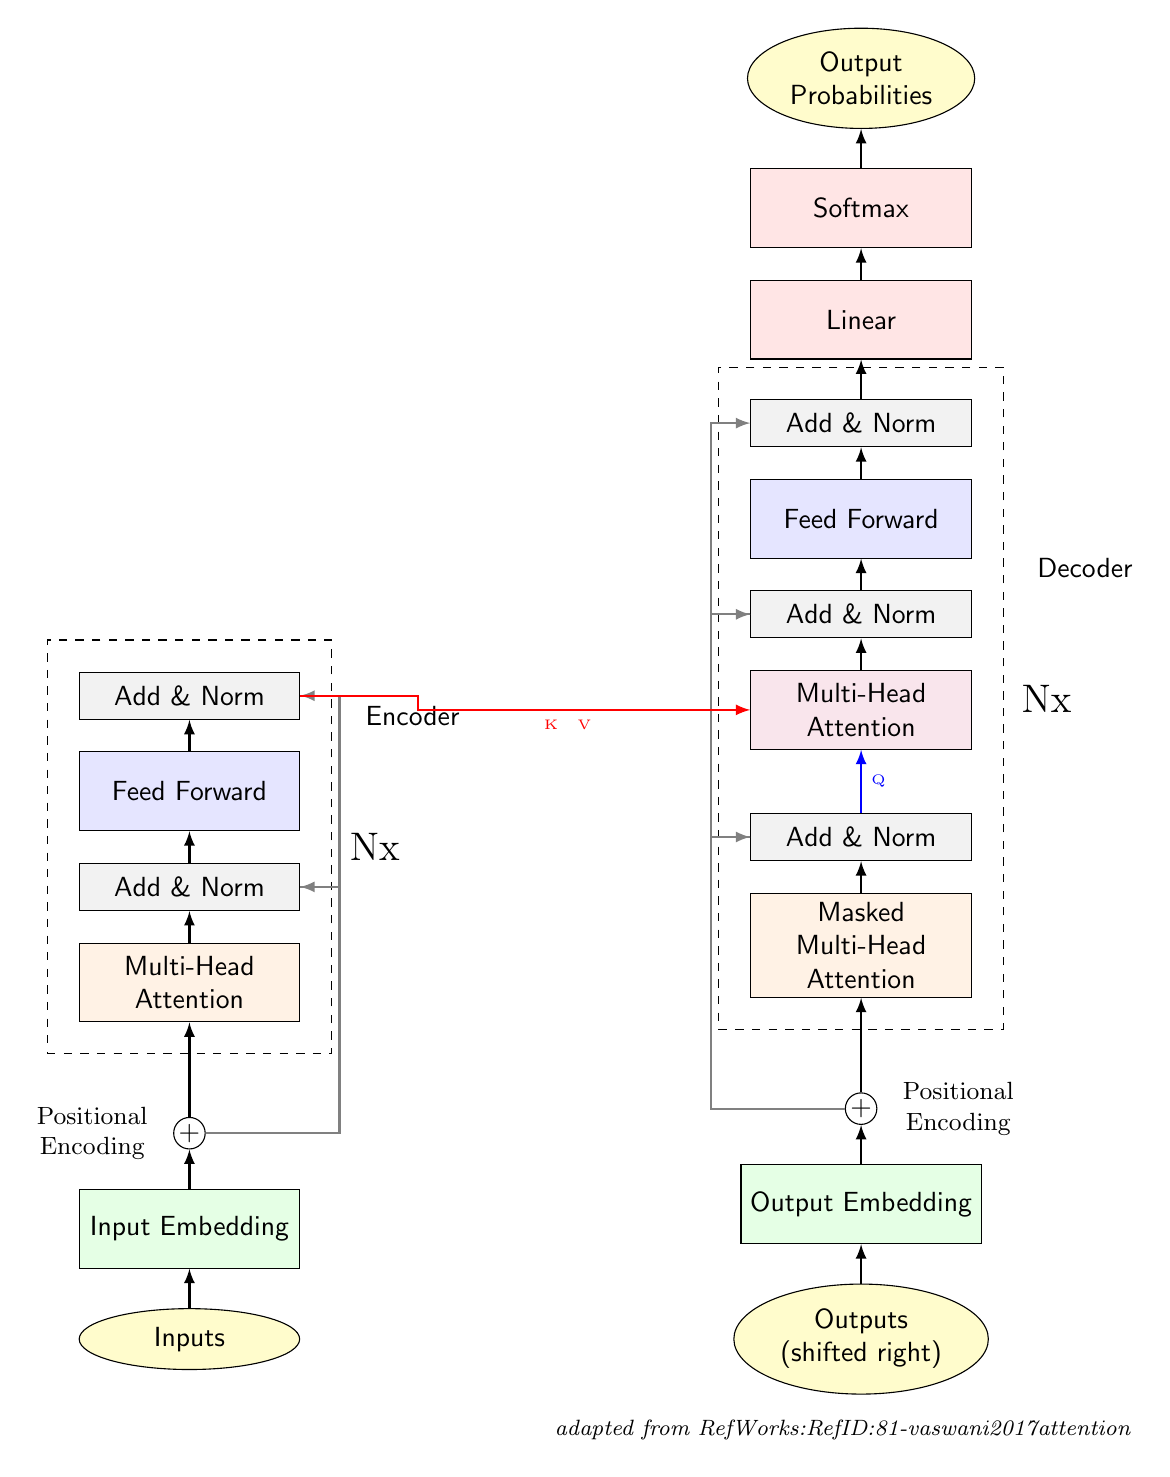
\begin{tikzpicture}[
    font=\sffamily,
    node distance=0.4cm,
    % Define styles for different types of nodes - with reduced widths
    block/.style={rectangle, draw, minimum width=2.8cm, minimum height=1cm, align=center},
    addnorm/.style={rectangle, draw, minimum width=2.8cm, minimum height=0.6cm, fill=gray!10},
    feedforward/.style={block, fill=blue!10},
    attention/.style={block, fill=orange!10},
    masked_attention/.style={attention},
    cross_attention/.style={attention, fill=purple!10},
    embedding/.style={block, fill=green!10, minimum height=1cm},
    softmax/.style={block, fill=red!10, minimum width=2.8cm},
    io/.style={ellipse, draw, fill=yellow!20, minimum width=2.8cm, align=center},
    plus/.style={circle, draw, inner sep=0pt, minimum size=0.4cm},
    connector/.style={-latex, thick},
    residual/.style={connector, gray},
    encoder_block_fit/.style={rectangle, draw, dashed, inner sep=0.4cm, label={[xshift=0.3cm, yshift=-0.4cm]above right:Encoder}},
    decoder_block_fit/.style={rectangle, draw, dashed, inner sep=0.4cm, label={[xshift=0.3cm, yshift=-0.4cm]above right:Decoder}}
]

%==============================================================================
% ENCODER SIDE (Left)
%==============================================================================

% Input nodes at the bottom
\node[io] (inputs) {Inputs};
\node[embedding, above=0.5cm of inputs] (input_embedding) {Input Embedding};
\node[plus, above=0.5cm of input_embedding] (pos_encoding_plus_in) {+};
% Repositioned label to the left to prevent overlap
\node[left=0.2cm of pos_encoding_plus_in, align=center, font=\small] (pos_encoding_in_label) {Positional\\Encoding};

% Encoder Stack
\node[attention, above=1.2cm of pos_encoding_plus_in] (enc_attention) {Multi-Head\\Attention};
\node[addnorm, above=0.4cm of enc_attention] (enc_addnorm1) {Add \& Norm};
\node[feedforward, above=0.4cm of enc_addnorm1] (enc_ff) {Feed Forward};
\node[addnorm, above=0.4cm of enc_ff] (enc_addnorm2) {Add \& Norm};

% Fit a box around the encoder stack
\node[encoder_block_fit, fit=(enc_attention) (enc_addnorm2)] (encoder_block) {};
\node[right=0.1cm of encoder_block, font=\Large] (enc_nx) {Nx};

%==============================================================================
% DECODER SIDE (Right)
%==============================================================================
\node[right=5.5cm of inputs] (outputs) [io] {Outputs \\ (shifted right)};
\node[embedding, above=0.5cm of outputs] (output_embedding) {Output Embedding};
\node[plus, above=0.5cm of output_embedding] (pos_encoding_plus_out) {+};
% Repositioned label to the right to prevent overlap
\node[right=0.2cm of pos_encoding_plus_out, align=center, font=\small] (pos_encoding_out_label) {Positional\\Encoding};

% Decoder Stack
\node[masked_attention, above=1.2cm of pos_encoding_plus_out] (dec_masked_attention) {Masked\\Multi-Head\\Attention};
\node[addnorm, above=0.4cm of dec_masked_attention] (dec_addnorm1) {Add \& Norm};
% Increased vertical spacing for Q line visibility
\node[cross_attention, above=0.8cm of dec_addnorm1] (dec_cross_attention) {Multi-Head\\Attention};
\node[addnorm, above=0.4cm of dec_cross_attention] (dec_addnorm2) {Add \& Norm};
\node[feedforward, above=0.4cm of dec_addnorm2] (dec_ff) {Feed Forward};
\node[addnorm, above=0.4cm of dec_ff] (dec_addnorm3) {Add \& Norm};

% Fit a box around the decoder stack
\node[decoder_block_fit, fit=(dec_masked_attention) (dec_addnorm3)] (decoder_block) {};
\node[right=0.1cm of decoder_block, font=\Large] (dec_nx) {Nx};

% Final output layers on top of decoder
\node[softmax, above=0.5cm of dec_addnorm3] (linear) {Linear};
\node[softmax, above=0.4cm of linear] (softmax) {Softmax};
\node[io, above=0.5cm of softmax] (output_probs) {Output\\Probabilities};

%==============================================================================
% CONNECTIONS
%==============================================================================

% --- Encoder Connections ---
\draw[connector] (inputs) -- (input_embedding);
\draw[connector] (input_embedding) -- (pos_encoding_plus_in);
\draw[connector] (pos_encoding_plus_in) -- (enc_attention);
\draw[connector] (enc_attention) -- (enc_addnorm1);
\draw[connector] (enc_addnorm1) -- (enc_ff);
\draw[connector] (enc_ff) -- (enc_addnorm2);

% --- Decoder Connections ---
\draw[connector] (outputs) -- (output_embedding);
\draw[connector] (output_embedding) -- (pos_encoding_plus_out);
\draw[connector] (pos_encoding_plus_out) -- (dec_masked_attention);
\draw[connector] (dec_masked_attention) -- (dec_addnorm1);
\draw[connector] (dec_cross_attention) -- (dec_addnorm2);
\draw[connector] (dec_addnorm2) -- (dec_ff);
\draw[connector] (dec_ff) -- (dec_addnorm3);
\draw[connector] (dec_addnorm3) -- (linear);
\draw[connector] (linear) -- (softmax);
\draw[connector] (softmax) -- (output_probs);

% --- Residual Connections ---
% Encoder
\draw[residual] (pos_encoding_plus_in.east) -| ++(1.7, 0) |- (enc_addnorm1.east);
\draw[residual] (enc_addnorm1.east) -| ++(0.5, 0) |- (enc_addnorm2.east);
% Decoder
\draw[residual] (pos_encoding_plus_out.west) -| ++(-1.7, 0) |- (dec_addnorm1.west);
\draw[residual] (dec_addnorm1.west) -| ++(-0.5, 0) |- (dec_addnorm2.west);
\draw[residual] (dec_addnorm2.west) -| ++(-0.5, 0) |- (dec_addnorm3.west);

% --- Encoder-to-Decoder Connections (Key/Value and Query) ---
% Red K,V line with more horizontal space to prevent overlap
\draw[connector, thick, red] (enc_addnorm2.east) -- ++(1.5, 0) |- node[pos=0.70, below, font=\tiny] {K} node[pos=0.75, below, font=\tiny] {V} (dec_cross_attention.west);

% Blue Q line is now a clean vertical path
\draw[connector, thick, blue] (dec_addnorm1.north) -- node[pos=0.5, right, font=\tiny] {Q} (dec_cross_attention.south);

% *** MODIFIED NODE FOR CITATION ***
% Positioned below the entire drawing at the right edge to avoid overlap.
\node[anchor=north east, font=\footnotesize, yshift=-0.2cm] at (current bounding box.south east)
    {\textit{adapted from \textcite{RefWorks:RefID:81-vaswani2017attention}}};
    
\end{tikzpicture}
\captionsetup{
    labelfont={bf,it},
    textfont=it,
}
% *** MODIFIED CAPTION ***
\captionsetup{
    labelfont={bf,it}, 
    textfont=it,  
    justification=centering
    }
\caption{\textit{The Transformer - model architecture}}
\label{fig:transformer}
\end{figure}

A fundamental limitation of LLMs, however, remains the context window size. This size, representing the maximum number of tokens the model can attend to simultaneously, is always finite, although it has increased with newer model generations \parencite{RefWorks:RefID:115-ratner2022parallel,RefWorks:RefID:100-kaplan2020scaling,RefWorks:RefID:99-liu2025comprehensive}. If a document's length exceeds this limit, the LLM cannot process it in a single pass. Standard techniques involve processing the document in chunks\index{Document Processing!chunking}, yet this can sever long-distance contextual links crucial for deep understanding \parencite{RefWorks:RefID:105-chen2024dense}. For example, determining if a policy defined on page one of a lengthy legal code is contradicted by regulations hundreds of pages later becomes impossible if the intervening text exceeds the context window, as the model would process these sections independently.

Furthermore, the computational cost of processing information within the context window is a significant factor. The self-attention mechanism, core to the Transformer, typically scales quadratically $(O(n^2))$\index{Attention Mechanism!computational complexity} with the sequence length $(n)$ in terms of both computation and memory requirements \parencite{RefWorks:RefID:81-vaswani2017attention}. Although various "efficient Transformer" variants aim to reduce this to near-linear complexity, processing long sequences still demands substantial resources \parencite{RefWorks:RefID:106-tay2023efficient}. This scaling makes analyzing very large documents prohibitively expensive or slow for many practical applications, further motivating alternative approaches, such as KG-based structuring, for achieving comprehensive and efficient analysis.

\subsection{The Challenge of Long-Context Processing}
\label{subsec:long_context}
While the Transformer architecture revolutionized NLP, its core self-attention mechanism presents a significant scalability challenge: a computational and memory cost that grows quadratically with the length of the input sequence \parencite{RefWorks:RefID:81-vaswani2017attention}. This creates a practical upper limit on the size of the context window, posing a major hurdle for processing lengthy documents. In response, researchers have pursued several strategies to mitigate this limitation. Architectural innovations such as sparse attention mechanisms (e.g., Longformer, BigBird) modify the attention matrix to attend to only a subset of tokens, thereby reducing the computational complexity from quadratic to near-linear \parencite{RefWorks:RefID:183-beltagylongformer,RefWorks:RefID:184-zaheerbig}. Other approaches, like Transformer-XL, introduce a recurrence mechanism that caches hidden states from previous segments, allowing information to flow beyond a fixed-size window \parencite{RefWorks:RefID:185-2019transformerxl}.

A more recent and widely adopted paradigm is Retrieval-Augmented Generation (RAG) \parencite{RefWorks:RefID:158-lewis2020retrievalaugmented}. In a RAG system, a large document corpus is first segmented into chunks and indexed in a vector database. When a query is posed, the system retrieves the most semantically relevant chunks and injects them into the LLM's context window as supplementary information for generating a response. While highly effective for knowledge-intensive tasks like question-answering, RAG is fundamentally oriented toward retrieving localized, salient information. It is less suited for tasks requiring a holistic, structural understanding of a document, such as verifying global consistency. For instance, to detect if a term defined in Chapter 1 is used in a contradictory manner in Chapter 20, a RAG system would have to coincidentally retrieve both specific, distant chunks in the same query, a scenario for which it is not optimized. This praxis contends that for comprehensive document validation, a pre-constructed Knowledge Graph, which explicitly models the entire document's entities and relationships, offers a more robust and systematically queryable structure than the on-the-fly, fragmented context provided by RAG.

\section{Knowledge Graphs}
Knowledge Graphs (KGs)\index{Knowledge Graphs} provide a structured paradigm for representing information, evolving from concepts in semantic networks\index{Semantic Networks}, frame systems\index{Knowledge Graphs!frames}, and earlier AI research in symbolic knowledge representation \parencite{RefWorks:RefID:102-hogan2021knowledge}. Formally, a KG represents knowledge as a directed labeled graph, comprising a collection of interconnected entities (nodes\index{Knowledge Graphs!nodes}) and the explicitly typed relationships (edges\index{Knowledge Graphs!edges}) between them. Both nodes and edges can possess attributes or properties that store additional metadata or context \parencite{RefWorks:RefID:108-ehrlinger2016definition, RefWorks:RefID:97-cong2024research}.

The core components of a KG are as follows:
\begin{itemize}
    \item \textbf{Nodes (Entities):}\index{Knowledge Graphs!nodes} These represent real-world objects, abstract concepts, events, or specific instances of interest. Examples include persons, organizations, locations, legal statutes ('15 Pa.C.S.A. § 1502'), or defined terms ('nonconforming use'). Nodes are often identified by unique identifiers.
    \item \textbf{Edges (Relationships):}\index{Knowledge Graphs!edges} These represent the connections or typed relationships between pairs of nodes, such as 'works for', 'located in', 'cites', or 'amends'. Edges are typically directed from a subject node to an object node and are labeled with the relationship type.
    \item \textbf{Attributes (Properties):}\index{Knowledge Graphs!attributes} These are key-value pairs associated with nodes or edges, providing additional details. For instance, a 'Person' node might have an 'email' attribute, or a 'cites' edge might have an 'effectiveDate' attribute.
\end{itemize}

\begin{figure}[H]
\centering
 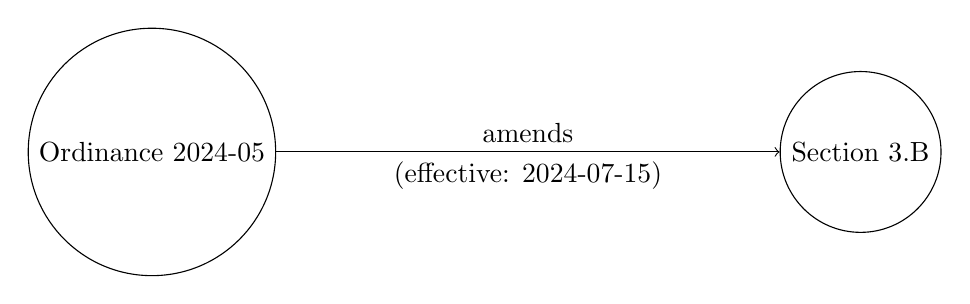
\begin{tikzpicture}[node distance={90mm}, main/.style = {draw, circle}]
 \node[main] (1) {Ordinance 2024-05};
 \node[main] (2) [right of=1] {Section 3.B};
 \draw[->] (1) -- node[midway, above] {amends} node[midway, below] {(effective: 2024-07-15)} (2);
\end{tikzpicture}
\captionsetup{
    labelfont={bf,it}, 
    textfont=it,  
    justification=centering
    }
\caption{Knowledge graph fragment of a legal amendment.}
\label{fig:simple_kg}
\end{figure}

Pioneering work in structured knowledge includes Minsky's concept of Frames\index{Minsky, Marvin}\index{Knowledge Graphs!frames}, which represented stereotypical situations using slots and relationships, thereby influencing subsequent formalisms like description logics and semantic web ontologies \parencite{RefWorks:RefID:78-minsky1974framework}.

\subsection{The Role of Ontologies and Schema in KG Construction}
\label{subsec:ontologies}
A Knowledge Graph's utility for analytical tasks extends beyond its raw structure of nodes and edges; it is deeply rooted in the formal schema, or ontology, that governs it. An ontology serves as the conceptual blueprint for the knowledge domain, explicitly defining the types of entities (classes), their attributes (properties), and the permissible relationships between them \parencite{RefWorks:RefID:135-noy2001ontology}. In the context of legal documents, an ontology might define classes such as \texttt{Ordinance}, \texttt{DefinedTerm}, and \texttt{ZoningDistrict}, along with rules specifying that an \texttt{Ordinance} can have an \texttt{enactmentDate} property of type \texttt{Date} and can be linked to a \texttt{DocumentSection} via an \texttt{AMENDS} relationship.

This formal specification is not merely a descriptive convenience; it is a prerequisite for automated validation. By defining a clear schema, one can programmatically check for both consistency and completeness. Consistency is checked by identifying graph structures that violate the ontological rules. For example, if a node representing a township is linked to a \texttt{PermittedUse} node, this would violate a schema rule stating that only \texttt{ZoningDistrict} nodes can have such a relationship. Completeness can be assessed against schema-defined cardinality constraints. If the ontology specifies that every \texttt{DefinedTerm} node \textit{must} have at least one incoming \texttt{DEFINES} relationship from a \texttt{DocumentSection} node, any such node lacking this relationship represents an instance of structural incompleteness within the KG, signaling a potential flaw in the source document. Thus, the ontology transforms the KG from a simple data structure into a formal model against which the document's integrity can be rigorously tested.

\subsection{Reasoning Over Knowledge Graphs}
\label{subsec:kg_reasoning}
The true analytical power of a Knowledge Graph is unlocked through reasoning—the process of inferring implicit knowledge from the explicitly asserted facts. Reasoning enables the discovery of relationships and properties that are not directly stated in the source text, allowing for a deeper and more comprehensive analysis. Two primary modes of reasoning are relevant to document validation: deductive and inductive.

Deductive reasoning uses a set of logical rules and axioms, often defined in the ontology, to derive new conclusions with certainty. Technologies like the Web Ontology Language (OWL) and the Shapes Constraint Language (SHACL) provide formalisms for expressing these rules \parencite{RefWorks:RefID:110-hitzler2009foundations, RefWorks:RefID:154-knublauch2017shapes}. For example, if the KG contains the facts (\texttt{Ordinance\_123}, \texttt{AMENDS}, \texttt{Section\_3.B}) and (\texttt{Section\_3.B}, \texttt{PART\_OF}, \texttt{Article\_III}), a deductive reasoner could apply a transitivity rule to infer the new triple (\texttt{Ordinance\_123}, \texttt{IMPACTS}, \texttt{Article\_III}). This capability is crucial for identifying the far-reaching consequences of amendments and for detecting logical contradictions that may only become apparent through multi-step inference.

Inductive reasoning, in contrast, is probabilistic and is typically performed using machine learning models that operate on graph structures, such as Graph Neural Networks (GNNs) \parencite{RefWorks:RefID:7-gupta2021graph}. A primary application of inductive reasoning in KGs is link prediction, where the model learns patterns from the existing graph structure to predict the likelihood of missing edges between nodes. In the context of document analysis, link prediction could identify a likely but absent \texttt{USES\_TERM} relationship between a section of text and a relevant defined term, flagging a potential omission for human review. While not logically certain, this inductive approach provides a powerful tool for identifying gaps and enhancing the completeness of the knowledge base.

\subsection{KG Technologies and Applications}
\label{subsec:kg_techandapp}

Knowledge graphs are implemented using various technologies. The Resource Description Framework (RDF)\index{Knowledge Graphs!RDF} is a W3C standard based on triples (subject-predicate-object) and is foundational to the Semantic Web\index{Semantic Web}. It is often queried using SPARQL\index{SPARQL} and defined with ontology languages like OWL\index{Ontology!OWL} \parencite{RefWorks:RefID:109-2025rdf, RefWorks:RefID:111-kumar2013querying, RefWorks:RefID:110-hitzler2009foundations}. Property Graphs\index{Knowledge Graphs!Property Graphs}, used in databases like Neo4j, offer a flexible model where both nodes and edges can have properties and are queried with languages like Cypher or Gremlin \parencite{RefWorks:RefID:114-fernandes2018graph}. Additionally, Graph Neural Networks (GNNs)\index{Graph Neural Networks (GNNs)} are machine learning techniques that operate on graph structures to learn vector representations (embeddings\index{Embeddings}), enabling tasks like link prediction and node classification \parencite{RefWorks:RefID:7-gupta2021graph, RefWorks:RefID:47-scarselli2009graph, RefWorks:RefID:49-wang2024graph}.

KGs are employed in diverse applications, including semantic search, recommendation systems, and enterprise data integration \parencite{RefWorks:RefID:102-hogan2021knowledge, RefWorks:RefID:118-ji2022survey, RefWorks:RefID:120-fensel2020knowledge}. Their ability to explicitly model complex relationships makes them valuable for analyzing the internal structure and integrity of large document collections.

\section{Information Extraction for KG Construction}
To leverage KGs for document analysis, the unstructured information within source documents must be transformed into the structured format of a graph. This process, termed KG construction\index{Knowledge Graphs!construction}, relies on Information Extraction (IE)\index{Information Extraction (IE)} techniques \parencite{RefWorks:RefID:121-zhong2024comprehensive, RefWorks:RefID:122-kolluru2020imojie}. This section covers two fundamental IE tasks: identifying nodes via Named Entity Recognition (NER)\index{Named Entity Recognition (NER)} and identifying edges via Relation Extraction (RE)\index{Relation Extraction (RE)}. LLMs have shown significant promise in performing both tasks, often with minimal task-specific training data \parencite{RefWorks:RefID:107-benjira2025automated}.

\subsection{Named Entity Recognition}
Named Entity Recognition (NER) is a primary task in information extraction that identifies and classifies named entities in text into predefined categories \parencite{RefWorks:RefID:4-al-moslmi2020named}. These categories can include standard types like persons and organizations or be extended to domain-specific entities. For building KGs, NER serves as the main mechanism for identifying the potential \textbf{nodes} of the graph. A subsequent step, Entity Linking\index{Entity Linking}, is often necessary to disambiguate these mentions and link them to unique identifiers \parencite{RefWorks:RefID:5-chaurasiya2022entity}.

NER methods have evolved significantly. Early approaches were rule-based systems\index{Named Entity Recognition (NER)!rule-based} that used hand-crafted rules and dictionaries, which achieved high precision but were brittle and labor-intensive \parencite{RefWorks:RefID:126-nadeau2007survey, RefWorks:RefID:127-grishman1996messageunderstanding}. These were followed by statistical models\index{Named Entity Recognition (NER)!statistical models} like Hidden Markov Models and Conditional Random Fields, which offered better generalization \parencite{RefWorks:RefID:128-lafferty2001conditional}. Currently, deep learning approaches\index{Named Entity Recognition (NER)!deep learning}, particularly Transformer-based models like BERT, have achieved state-of-the-art performance by leveraging powerful pre-trained representations \parencite{RefWorks:RefID:4-al-moslmi2020named, RefWorks:RefID:57-carbonell2020named}.

Applying NER to the legal domain requires identifying specialized entities such as specific statutes, defined legal terms, legal roles, and explicit document references \parencite{RefWorks:RefID:124-au2022ener, RefWorks:RefID:125-kalamkar2022named}. The unique vocabulary and complex sentence structures of legal texts necessitate that NER models be trained or fine-tuned on legally annotated corpora to achieve high accuracy \parencite{RefWorks:RefID:64-2022lexglue}. A robust legal NER system provides the essential building blocks for constructing a meaningful knowledge graph from legal documents.

\subsection{Relation Extraction}
While NER identifies entities (nodes), Relation Extraction (RE)\index{Relation Extraction (RE)} identifies the semantic relationships between them, which correspond to the edges in a knowledge graph \parencite{RefWorks:RefID:118-ji2022survey, RefWorks:RefID:57-carbonell2020named}. For instance, from the sentence "Acme Corp, headquartered in West Chester, acquired Beta Inc.," RE aims to identify relations such as `headquarteredIn(Acme Corp, West Chester)`. This task is crucial for building the graph's structure. Work in this area includes both Closed RE, for a predefined set of relation types, and Open Information Extraction (OpenIE)\index{Information Extraction (IE)!OpenIE}, which extracts relations expressed with arbitrary text \parencite{RefWorks:RefID:134-etzioni2008acm}.

Approaches to RE have mirrored those in NER. Early systems were rule-based\index{Relation Extraction (RE)!rule-based}, using linguistic patterns to identify relations \parencite{RefWorks:RefID:136-hearst1992automatic}. Supervised statistical models\index{Relation Extraction (RE)!statistical models} followed, using classifiers trained on annotated data or data generated through distant supervision\index{Relation Extraction (RE)!distant supervision}, a technique that aligns known relations from KGs with text but can introduce noise \parencite{RefWorks:RefID:139-kambhatla2004combining, RefWorks:RefID:140-mintz2009distant}. Modern deep learning approaches\index{Relation Extraction (RE)!deep learning}, especially Transformer-based models, now represent the state-of-the-art \parencite{RefWorks:RefID:141-kumar2017survey, RefWorks:RefID:142-wu2019enriching}. LLMs, through prompting techniques, offer a powerful alternative capable of extracting relations with minimal task-specific fine-tuning \parencite{RefWorks:RefID:143-chia2022relation}.

Key challenges in RE include handling ambiguity, extracting relations that span sentences, and adapting models to new domains. In the legal context, extracting relations such as amendments, definitions, and obligations is critical for building a KG that accurately reflects the legal framework \parencite{RefWorks:RefID:77-tauqeer2022automated, RefWorks:RefID:76-dhani2021similar}. The structured output from NER and RE forms the basis for the constructed knowledge graph.

\section{Consistency, Completeness, and Coherence}
When analyzing formal document corpora such as legal codes or technical standards, quality evaluation often involves assessing internal integrity. Three key aspects of this integrity are consistency\index{Consistency}, completeness\index{Completeness}, and coherence\index{Coherence} \parencite{RefWorks:RefID:29-umar2024advances}. These concepts, while sometimes overlapping, address distinct facets crucial for ensuring documents are understandable, unambiguous, and effective.

\begin{itemize}
    \item \textbf{Consistency:}\index{Consistency} Refers to the absence of logical contradictions within a document set \parencite{RefWorks:RefID:10-zowghi2003interplay, RefWorks:RefID:21-heitmeyer1996automated, RefWorks:RefID:25-nentwich2005managing, RefWorks:RefID:26-egyed2006instant, RefWorks:RefID:27-tröls2022instant, RefWorks:RefID:28-yang2024fizz, RefWorks:RefID:30-guo2023joint}. A consistent document should not contain provisions that assert mutually exclusive facts or prescribe conflicting obligations under identical conditions. Detecting such inconsistencies is vital for legal certainty and predictability \parencite{RefWorks:RefID:52-donelson2019legal, RefWorks:RefID:53-duck-mayr2022explaining, RefWorks:RefID:54-rossi2016inconsistent}. Formal logic and automated reasoning techniques are often employed to check consistency in formal specifications \parencite{RefWorks:RefID:21-heitmeyer1996automated, RefWorks:RefID:24-brucker2019ontologies}.

    \item \textbf{Completeness:}\index{Completeness} Pertains to whether the document set contains all necessary information relative to its intended scope \parencite{RefWorks:RefID:10-zowghi2003interplay}. Defining completeness is inherently challenging, as it depends on a clear specification of what should be included. In a legal context, completeness may require that all terms are adequately defined, referenced procedures are specified, and relevant scenarios are addressed. Gaps or omissions can lead to ambiguity and disputes. Assessing completeness often requires significant domain knowledge and may involve checking against predefined templates or requirements specifications \parencite{RefWorks:RefID:10-zowghi2003interplay, RefWorks:RefID:29-umar2024advances}. The interpretation of completeness in KGs is also affected by the "Closed World Assumption" versus the "Open World Assumption"\index{Knowledge Graphs!reasoning!Closed World Assumption} \parencite{RefWorks:RefID:148-reiter1978on, RefWorks:RefID:110-hitzler2009foundations}.

    \item \textbf{Coherence:}\index{Coherence} Relates to the overall understandability, organization, and logical flow of the presented information \parencite{RefWorks:RefID:44-wang2014short, RefWorks:RefID:14-shen2021evaluating}. A coherent document is well-structured, uses terminology consistently, and ensures cross-references are accurate. While related to consistency, coherence focuses more on clarity and comprehensibility for a human reader, encompassing aspects like lexical cohesion and discourse structure \parencite{RefWorks:RefID:44-wang2014short}.
\end{itemize}

Ensuring these three qualities simultaneously in large, evolving legal codes through traditional manual review is exceptionally difficult. The volume of text, the intricate web of interdependencies, the potential for ambiguity in natural language, and the distributed nature of authorship make manual detection of subtle flaws challenging and error-prone \parencite{RefWorks:RefID:68-beth2018bills}. Computational approaches that leverage structured representations like KGs offer significant potential advantages.

A Knowledge Graph provides a structured substrate amenable to automated analysis by explicitly modeling entities and their relationships. Graph-based queries and algorithms can be designed to automatically detect potential inconsistencies, such as conflicting property values or circular definition chains \parencite{RefWorks:RefID:77-tauqeer2022automated, RefWorks:RefID:24-brucker2019ontologies, RefWorks:RefID:19-schönberg2011verifying, RefWorks:RefID:23-weitl2006checking}. While perfect completeness verification is often intractable for natural language documents, KGs can help identify potential gaps by analyzing the graph's structure for missing nodes, absent relationships, or orphaned sections \parencite{RefWorks:RefID:151-rabbani2023extraction, RefWorks:RefID:152-rabbani2022shacl, RefWorks:RefID:153-omran2020shacl, RefWorks:RefID:154-knublauch2017shapes, RefWorks:RefID:29-umar2024advances}.

LLMs can play a role throughout this pipeline, aiding in the initial interpretation of text to populate the KG, helping to formulate complex graph queries, or summarizing the findings from the analysis for human review \parencite{RefWorks:RefID:107-benjira2025automated}. The KG itself, however, provides the persistent, globally coherent, and computationally tractable structure necessary for systematic integrity checks. Such a structure can overcome the context window limitations and potential lack of deterministic reasoning inherent in LLMs alone. Research exploring KGs and related AI techniques for automated integrity checking provides a foundation for this approach \parencite{RefWorks:RefID:29-umar2024advances, RefWorks:RefID:21-heitmeyer1996automated, RefWorks:RefID:77-tauqeer2022automated, RefWorks:RefID:76-dhani2021similar, RefWorks:RefID:11-aumiller2021structural}. This praxis project aims to build upon such work by investigating the practical application of LLM-driven KG construction for analyzing municipal legal codes.

\section{Challenges in Analyzing Large Documents} \label{sec:doc_processing}
Research in automated document processing is extensive, covering tasks like summarization, information extraction, and question answering \parencite{RefWorks:RefID:156-gambhir2017recent, RefWorks:RefID:121-zhong2024comprehensive, RefWorks:RefID:157-2017reading}. Historically, much of this research focused on relatively small documents, as they are less computationally demanding and more feasible for the human evaluation required to establish ground truth.

Many critical real-world applications, however, involve documents that are orders of magnitude larger, such as legal contracts, technical manuals, and extensive regulatory codes. Analyzing these large documents\index{Document Processing!large documents} presents distinct and significant challenges:
\begin{itemize}
    \item \textbf{Computational Resources:}\index{Document Processing!large documents!computational resources} Processing large volumes of text demands substantial memory, storage, and processing time. The computational complexity often scales non-linearly with document length, making naive processing of entire large documents infeasible \parencite{RefWorks:RefID:81-vaswani2017attention}.
    \item \textbf{Long-Range Dependencies:}\index{Document Processing!large documents!long-range dependencies} Comprehension frequently requires capturing semantic connections or references between sections that are far apart in the document. Models with limited context windows struggle to capture these long-distance relationships accurately \parencite{RefWorks:RefID:99-liu2025comprehensive, RefWorks:RefID:101-zhao2023survey}.
    \item \textbf{Context Fragmentation:}\index{Document Processing!large documents!context fragmentation} A common technique for handling large documents involves splitting them into smaller chunks. This method, while necessary for models with fixed inputs, risks losing critical context that spans chunk boundaries, potentially leading to fragmented understanding \parencite{RefWorks:RefID:105-chen2024dense, RefWorks:RefID:104-qu2024semantic}.
    \item \textbf{Evaluation Complexity:}\index{Document Processing!large documents!evaluation complexity} Assessing the quality of automated analysis on a large document is inherently difficult for human evaluators. Establishing reliable ground truth for evaluation benchmarks remains a major challenge for large-document tasks \parencite{RefWorks:RefID:116-shaham2022scrolls}.
\end{itemize}
Techniques like Retrieval-Augmented Generation (RAG)\index{Retrieval-Augmented Generation (RAG)} allow LLMs to leverage information from large external corpora without processing the entire corpus in their context window \parencite{RefWorks:RefID:158-lewis2020retrievalaugmented}. RAG retrieves relevant text snippets and provides them as context to the LLM. Although powerful for knowledge-intensive tasks, standard RAG retrieves discrete, localized chunks and may not provide the holistic, structured view of the entire document that a pre-constructed Knowledge Graph can offer.

\section{Challenges in Analyzing Legal Documents} \label{sec:legal_docs}
Legal documents, particularly statutory codes, represent a compelling yet challenging domain for advanced document analysis techniques. They possess several intrinsic characteristics that make them difficult testbeds and valuable targets for automation:\index{Legal Document Analysis}
\begin{itemize}
    \item \textbf{Complexity and Precision:}\index{Legal Document Analysis!complexity and precision} Legal language is dense, employing specialized terminology and complex sentence structures. Ambiguity must be minimized, demanding high precision in interpretation, as misinterpretations can have significant real-world consequences \parencite{RefWorks:RefID:159-ashley2017artificial, RefWorks:RefID:62-malik2022semantic}.
    \item \textbf{Volume and Interconnectedness:}\index{Legal Document Analysis!volume and interconnectedness} Legal corpora can be vast and are highly interconnected through citations, amendments, and definitions. Understanding one part often requires understanding its relationship to many others \parencite{RefWorks:RefID:68-beth2018bills}.
    \item \textbf{Semi-structured Format:}\index{Legal Document Analysis!semi-structured format} Legal texts mix structured elements (e.g., sections, clauses) with unstructured natural language prose, requiring sophisticated NLP techniques to handle both.
    \item \textbf{Critical Need for Integrity:}\index{Legal Document Analysis!integrity} The consistency, completeness, and coherence of legal documents are paramount for their function. These qualities underpin the rule of law, ensuring predictability and enforceability. Flaws can lead to disputes, costly litigation, and erosion of public trust \parencite{RefWorks:RefID:52-donelson2019legal, RefWorks:RefID:53-duck-mayr2022explaining, RefWorks:RefID:54-rossi2016inconsistent}.
\end{itemize}

The specific focus on the codified ordinances of Pennsylvania townships provides a valuable and concrete dataset. These codes exhibit realistic complexity, having often been developed over decades with multiple authorships and numerous amendments. The legislative drafting and codification process, although designed to ensure quality through multi-stage human review, can still introduce errors. Inconsistencies, incompleteness, and incoherence can persist as the code grows \parencite{RefWorks:RefID:54-rossi2016inconsistent}. The resource-intensive and fallible nature of purely manual review motivates the exploration of computational methods to assist legal professionals in maintaining the integrity of these foundational legal documents.

\section{Related Work} % Needs to be filled with actual citations
Research relevant to this praxis project spans several areas: utilizing LLMs for Information Extraction, applying KGs for document integrity checking, and the application of NLP to the legal domain.

\textbf{LLMs for Information Extraction and KG Construction:}\index{Information Extraction (IE)!using LLMs}\index{Knowledge Graphs!construction!using LLMs}
The advent of powerful LLMs has advanced information extraction. Studies demonstrate the ability of models like GPT-4, often via prompting, to perform NER and RE with performance rivaling or exceeding traditional fine-tuned models, especially in specialized domains \parencite{RefWorks:RefID:160-xu2024large}. Researchers have explored various techniques to mitigate LLM limitations like hallucinations\index{Large Language Models (LLMs)!hallucinations} and to control output structure \parencite{RefWorks:RefID:87-wang2023gptner}. Several works focus on constructing KGs from text using LLMs as the primary extraction engine, developing pipelines that integrate entity identification, relation extraction, and schema mapping, sometimes with human-in-the-loop refinement \parencite{RefWorks:RefID:107-benjira2025automated, RefWorks:RefID:162-lairgi2024knowledge}.

\textbf{KGs for Document Analysis and Integrity Checking:}\index{Knowledge Graphs!for document analysis}
Beyond construction, KGs serve as a substrate for advanced document analysis, including semantic search and complex question answering \parencite{RefWorks:RefID:102-hogan2021knowledge, RefWorks:RefID:118-ji2022survey}. Directly relevant to this work is the use of KGs for consistency and completeness checking. In software requirements engineering, KGs and ontologies model requirements to detect conflicts \parencite{RefWorks:RefID:29-umar2024advances}. In the Semantic Web community, technologies like SHACL (Shapes Constraint Language)\index{SHACL (Shapes Constraint Language)} provide a standard way to validate RDF KGs against predefined constraints, effectively checking aspects of data integrity \parencite{RefWorks:RefID:154-knublauch2017shapes}.

\textbf{AI and NLP for Legal Document Analysis:}\index{Legal Document Analysis}
The legal domain has been a target for AI and NLP research for decades \parencite{RefWorks:RefID:159-ashley2017artificial}. Recent research applies modern NLP to tasks like legal information retrieval, case outcome prediction, and contract review \parencite{RefWorks:RefID:45-moens2001innovative, RefWorks:RefID:164-aletras2016predicting, RefWorks:RefID:64-2022lexglue}. Information extraction from legal texts has received significant attention, focusing on extracting citations, legal entities, and obligations \parencite{RefWorks:RefID:125-kalamkar2022named, RefWorks:RefID:77-tauqeer2022automated}. Some prior work has explored automated consistency checking in legal documents, often using rule-based or logic-based approaches, but these efforts have typically focused on specific types of conflicts rather than a comprehensive KG-based approach applied to municipal codes \parencite{RefWorks:RefID:54-rossi2016inconsistent}.

\subsection{Unique Linguistic Features of Legal Text}
\label{subsec:legal_linguistics}
The analysis of legal documents constitutes a distinct and challenging subfield of NLP, often referred to as Legal AI, due to the unique linguistic register, or "legalese," employed in these texts \parencite{RefWorks:RefID:159-ashley2017artificial}. This register presents formidable obstacles for standard NLP models that are typically trained on general-domain corpora. Key features include:

\begin{itemize}
    \item \textbf{Deontic Modality:} Legal texts are saturated with the language of obligations, permissions, and prohibitions, expressed through modal verbs such as \textit{shall}, \textit{must}, \textit{may}, and \textit{is prohibited} \parencite{RefWorks:RefID:186-navarro2014deontic}. Accurately parsing these expressions to extract the agent (who is obligated), the action (what must be done), and the specific modal force is essential for modeling the regulatory framework encoded in the text.
    \item \textbf{Intertextuality:} Legal documents rarely exist in isolation. Their meaning is constructed through a dense web of internal and external citations, such as ``as defined in Section 3.B'' or ``pursuant to 53 Pa.C.S.A. § 101''. This high degree of intertextuality means that a document's semantic content is distributed across multiple locations, making the modeling of these referential links—an inherently graph-like problem—paramount for any coherent analysis.
    \item \textbf{Controlled Vocabulary and Ambiguity:} While legal language strives for precision through a controlled vocabulary of defined terms, it is also rife with potential ambiguity. Syntactic ambiguity can arise from complex sentence structures with long, nested clauses, making it difficult to determine the scope of modifiers (the "dangling else" problem). Semantic ambiguity can occur when a term has a specific legal meaning that differs from its common usage.
\end{itemize}
These unique challenges necessitate specialized NLP approaches that can move beyond simple entity recognition to a more nuanced extraction of structured legal rules, definitions, and deontic relationships.

\subsection{A Brief History of Computational Law}
\label{subsec:legal_ai_history}
The application of computational methods to legal text is not a new endeavor; the field of Computational Law has evolved over several decades, mirroring broader trends in artificial intelligence. Understanding this history provides context for the contemporary approaches leveraged in this praxis.

The earliest forays into Legal AI, beginning in the 1970s and 1980s, were dominated by rule-based expert systems \parencite{RefWorks:RefID:187-susskind1986expert}. These systems attempted to capture legal knowledge by having human experts manually encode statutes and case law into formal logic, often using languages like Prolog. While pioneering, these systems were brittle, struggled to handle legal ambiguity, and faced an insurmountable "knowledge acquisition bottleneck," as the manual encoding process was extraordinarily labor-intensive.

The subsequent era saw a shift toward statistical methods and the rise of large-scale legal databases like Westlaw and LexisNexis. The primary focus of NLP during this period was on Legal Information Retrieval (LIR), using techniques from information retrieval to improve the search and discovery of relevant documents for legal professionals. This period also saw the application of machine learning to tasks such as e-discovery, where algorithms were used to classify documents as relevant or non-relevant to a case, drastically reducing the burden of manual review.

The modern era of Computational Law is defined by the advent of deep learning and, most recently, Large Language Models. Transformer-based models have achieved state-of-the-art results on a variety of legal tasks, including predicting judicial decisions from case texts \parencite{RefWorks:RefID:164-aletras2016predicting}, automated summarization of legal opinions, and the analysis and clause extraction from contracts. The research presented in this praxis is situated within this modern paradigm, applying the powerful generative and analytical capabilities of LLMs to the foundational but often-overlooked task of ensuring the internal structural integrity of the legislative documents that form the basis of the rule of law.

\textbf{Positioning of this Work:}
This praxis project builds upon these converging lines of research. While previous work has explored LLMs for KG construction and KGs for consistency checking separately, the specific contribution here lies in the integration and practical application of modern LLMs to construct KGs from municipal legal codes for consistency and completeness analysis. The project addresses LLM context window limitations by leveraging the KG structure for global reasoning. Unlike prior legal AI work focusing on case law or contracts, this project targets foundational legislative texts at the local government level. The "praxis" aspect emphasizes developing and evaluating a practical methodology to assist municipal professionals in maintaining the quality of their codified laws.

\section{Conclusions}

This review of the literature establishes a foundational tension in modern NLP: while Large Language Models built on the Transformer architecture possess unprecedented text processing capabilities, their inherent context window limitations prevent the holistic analysis required for verifying the integrity of large documents \parencite{RefWorks:RefID:81-vaswani2017attention, RefWorks:RefID:99-liu2025comprehensive}. The research surveyed demonstrates that Knowledge Graphs (KGs) present a robust solution to this challenge by transforming unstructured text into a persistent, structured, and globally queryable representation of knowledge \parencite{RefWorks:RefID:102-hogan2021knowledge}.

The process of Information Extraction, encompassing Named Entity Recognition (NER) and Relation Extraction (RE), serves as the critical bridge between the unstructured document and the structured KG \parencite{RefWorks:RefID:160-xu2024large}. By leveraging a KG, the core quality attributes of a document—\textbf{consistency}, \textbf{completeness}, and \textbf{coherence}—are made computationally tractable. This allows for systematic analysis that can overcome the limitations of manual review, which is particularly error-prone in dense, interconnected legal corpora \parencite{RefWorks:RefID:10-zowghi2003interplay, RefWorks:RefID:68-beth2018bills}.

While the literature addresses LLM-driven knowledge extraction, KG-based analysis, and Legal AI as separate fields, this project is situated at their practical synthesis. The novel contribution of this work is the integration of these techniques into a single framework focused specifically on analyzing the structural integrity of municipal legal codes. The limitations of current models and the critical need for reliable legal frameworks, as established in this review, directly motivate the methodology of this praxis project. The following chapter will detail the specific methodology employed to construct and evaluate a system designed to achieve this objective.
  
%%%%%%%%%%%%%%%%%%%%%%%%%%%%%%%%%%%%%%%%%%%%%%%%%%%%%%%%%%%%%%%%%%%%%%%%%%%%%%%
% CHAPTER 3: Methodology
%       DUE: July 1, 2025
%     PAGES: 25-30
%%%%%%%%%%%%%%%%%%%%%%%%%%%%%%%%%%%%%%%%%%%%%%%%%%%%%%%%%%%%%%%%%%%%%%%%%%%%%%%
\chapter{Methodology}
\label{chap:methodology}

\section{Introduction}
This chapter details the systematic methodology for developing and evaluating a system that leverages Large Language Models (LLMs) to convert extensive legal documents into attributed knowledge graphs (KGs) \parencite{RefWorks:RefID:102-hogan2021knowledge, RefWorks:RefID:120-fensel2020knowledge}. As established in Chapter 1, these KGs are intended to serve as a foundation for subsequent analysis of document completeness and consistency \parencite{RefWorks:RefID:10-zowghi2003interplay, RefWorks:RefID:29-umar2024advances}. The challenge of managing the complexity and scale of modern textual documents, particularly in legal codification, necessitates automated solutions \parencite{RefWorks:RefID:165-bhattacharya2019comparative}. Traditional manual review is often insufficient for ensuring comprehensive consistency in large, evolving document sets. This research posits that KGs, by providing structured representations of entities and their relationships, offer a viable approach to address these challenges \parencite{RefWorks:RefID:121-zhong2024comprehensive}.

The methodology herein is designed to be rigorous and reproducible. It outlines the overall research approach, system architecture, and data sources—specifically, Pennsylvania township laws. The chapter then details the critical hyperparameters governing the system, the experimental plan for their tuning, the software tools utilized, and the multi-faceted strategy for evaluating the quality of the generated KGs in the absence of a definitive ground truth. Finally, the inherent limitations of the chosen methods and relevant ethical considerations are examined, concluding with a restatement of the research questions and hypotheses this framework aims to address.

\section{Approach}
This research introduces Mnemosyne, a novel, multi-stage pipeline for transforming large, complex legislative documents into queryable Knowledge Graphs (KGs). Hereafter, this system will be referred to as Mnemosyne. By leveraging Large Language Models (LLMs) \parencite{RefWorks:RefID:107-benjira2025automated, RefWorks:RefID:162-lairgi2024knowledge}, our system is designed to facilitate automated analysis of legal texts for internal consistency and completeness. The architecture prioritizes two critical features: usability, requiring minimal specialized skill for operation, and traceability, ensuring every piece of information in the KG can be precisely linked to its source sentence. While developed using legal corpora, the modular design is generalizable to other domains characterized by large, structured documents \parencite{RefWorks:RefID:116-shaham2022scrolls}.

\subsection{Architectural Overview}
The system employs a modular pipeline that synthesizes established KG construction practices \parencite{RefWorks:RefID:118-ji2022survey} with a novel, two-tiered memory architecture adapted for the legal domain. This design manages the inherent complexity and context window limitations of modern LLMs \parencite{RefWorks:RefID:99-liu2025comprehensive} by building the KG iteratively. The data flows through a sequence of components, from initial document processing to advanced semantic enrichment. This modularity permits targeted optimization and evaluation at each stage. \Cref{fig:proposed_architecture} provides a high-level depiction of this data flow.

\begin{figure}[htbp]
    \centering
    \includegraphics[width=\linewidth]{figures/chap3_fig/Proposed Architecture.png}
    \captionsetup{
        labelfont={bf,it}, 
        textfont=it, 
        justification=centering
    }
    \caption{High-Level Overview of the Document-to-KG Pipeline}
    \label{fig:proposed_architecture}
\end{figure}

\subsubsection{Document Ingestion and Chunking (P1)}
The pipeline begins by ingesting source documents and segmenting them into semantically coherent units, or \textit{chunks}. This chunking process is a critical preprocessing step to overcome the fixed context window of LLMs. A naive split can sever key semantic links; therefore, this component implements and evaluates several intelligent strategies, including fixed-size token windows, paragraph-based segmentation, and overlapping chunks. For hierarchically structured legal documents, a structure-aware strategy leverages the heading styles in DOCX files to ensure chunks do not violate logical boundaries (e.g., articles, sections). Each chunk is meticulously annotated with location metadata (e.g., page, section number) to guarantee end-to-end traceability.

While a fixed-size token window is computationally simple, it risks arbitrarily severing legal clauses and definitions, thereby destroying semantic context. Paragraph-based segmentation is an improvement, but legal paragraphs can vary dramatically in length. Our primary approach, a structure-aware strategy, leverages the hierarchical nature of DOCX files by identifying heading styles (e.g., 'Heading 1' for Articles, 'Heading 2' for Sections). This method ensures that chunks correspond to logical divisions in the law, preserving the integrity of individual provisions. To mitigate context loss at the boundaries, we will experiment with an overlapping chunk mechanism, where the last 1-2 sentences of a chunk are repeated at the beginning of the next.

\subsubsection{Justification for Structure-Aware Chunking}
The selection of a chunking strategy is not merely a technical preprocessing step; it is a critical decision that directly impacts the semantic integrity of the data fed to the LLM. While simpler methods like fixed-size token windows offer computational efficiency and predictability, they are fundamentally agnostic to the document's underlying logical structure. In a domain like law, where the precise scope of a clause or definition is paramount, arbitrarily splitting a sentence can lead to catastrophic context loss. For example, a sentence specifying an exception to a rule might be split from the rule itself, leading the LLM to misinterpret the rule as absolute.

Paragraph-based chunking offers an improvement by respecting basic prose boundaries. However, legal documents often contain paragraphs of vastly different lengths, from single-line definitions to dense, multi-sentence regulatory requirements. This can result in chunks that are either too small to provide sufficient context or too large to fit within the LLM's context window.

Our choice of a \textbf{structure-aware strategy} is therefore justified by the nature of the legal corpus itself. By leveraging the explicit hierarchical metadata embedded in DOCX files (e.g., heading styles for Articles, Sections, and Subsections), we create chunks that correspond to discrete, logical units of law. This method presumes that the document's authors used these structural elements to delineate self-contained ideas. This alignment between the chunk and the logical unit maximizes the semantic context available to the LLM for each processing task, thereby minimizing the risk of misinterpretation at the foundational stage of knowledge extraction. The trade-off is a dependency on well-structured source documents, a limitation addressed in Section 3.10.

\subsubsection{LLM-Based Information Extraction (P3)}
This component serves as the core information extraction engine. For each text chunk, a carefully engineered prompt instructs an LLM to perform two coordinated tasks: Named Entity Recognition (NER) and Relation Extraction (RE). The model identifies entities corresponding to a predefined legal ontology (e.g., \texttt{Ordinance}, \texttt{DefinedTerm}, \texttt{ZoningDistrict}) and the semantic relationships between them (e.g., \texttt{AMENDS}, \texttt{DEFINES}, \texttt{PERMITS\_IN}). To ensure structured, reliable output, the LLM’s generation is constrained to a predefined JSON schema. The result for each chunk is a self-contained KG fragment, a design that enables parallel processing for enhanced throughput.

The efficacy of component P3 is highly dependent on prompt design. We will employ a few-shot prompting strategy. Each prompt sent to the LLM will include not only the text chunk to be analyzed but also 2-3 canonical examples of correctly extracted entities and relations. This guides the model towards the desired output format and legal ontology. Furthermore, the prompt will explicitly instruct the model to adhere to the provided JSON schema, a technique known as 'schema-constrained generation,' to minimize output errors and streamline parsing.

\subsubsection{Short-Term Memory (STM): Batch Aggregation (KG1)}
As KG fragments are generated, they are temporarily held in the Short-Term Memory (STM), an in-memory buffer. The STM functions as an efficient staging area, accumulating fragments until a predefined batch size is reached (the "STM fullness threshold" hyperparameter). This batching strategy optimizes performance by reducing the I/O overhead associated with numerous small writes to the persistent database. It also creates an opportunity for low-cost, preliminary consolidation operations before committing the data to long-term storage.

\subsubsection{LTM Ingestion and Entity Resolution (P4 \& KG2)}
Once the STM reaches capacity, the Long-Term Memory (LTM) Ingestion process is triggered. This blocking operation transfers the batch of KG fragments from the STM into the persistent graph database, which constitutes the LTM. The LTM is implemented in Neo4j, a database optimized for highly interconnected data. A crucial step in this process is \textit{entity resolution}, which de-duplicates nodes by merging new entities with existing ones based on unique identifiers or high lexical similarity. For example, multiple mentions of ``Ordinance 2024-05'' are resolved into a single canonical node. This ensures the global KG remains consistent and serves as the definitive, structured representation of the source documents.

Entity resolution in P4 is a multi-step process. For entities with explicit identifiers, such as an ordinanceNumber, resolution is a straightforward merge operation. For entities without unique IDs, such as DefinedTerm, we employ a hybrid approach. Initially, nodes are merged based on high lexical similarity (e.g., a Levenshtein distance below a certain threshold). In the subsequent asynchronous refinement stage (P5), we will further refine this by comparing the vector embeddings of potentially duplicate nodes. Nodes with a cosine similarity above a tuned threshold (e.g., 0.95) will be merged, ensuring that semantically identical concepts are represented by a single canonical node.

\subsubsection{Asynchronous KG Refinement and Enrichment (P5)}
The final stage is an asynchronous engine that performs computationally intensive refinement operations to enhance the global KG's semantic richness. This process operates iteratively on small, random subsets of the graph, allowing the KG to improve gradually without blocking ingestion or requiring complete reprocessing. This stage is triggered only when the primary ingestion pipeline is idle. Key operations include:
\begin{itemize}
    \item \textbf{Ontological Classification:} Formalizing type hierarchies by asserting \texttt{ISA} relationships (e.g., "Ordinance\_123" \texttt{ISA} "Ordinance"), essential for semantic reasoning \parencite{RefWorks:RefID:135-noy2001ontology, RefWorks:RefID:78-minsky1974framework}.
    \item \textbf{Meronymic Relationship Modeling:} Establishing the document's structure within the graph by adding part-whole (\texttt{PARTOF}) relationships (e.g., "Section\_3.B" \texttt{PARTOF} "Article\_III").
    \item \textbf{Type System Refinement:} Identifying and merging semantically equivalent entity types (e.g., consolidating "Regulation" and "Rule") by calculating the similarity of their LLM-generated embeddings \parencite{RefWorks:RefID:167-gardazi2025bert}.
    \item \textbf{Ontology Organization:} Structuring entity types into a coherent subsumption hierarchy using a combination of LLM-based classification and domain heuristics \parencite{RefWorks:RefID:6-2022knowledge}.
    \item \textbf{Instance Type Correction:} Re-classifying entity instances based on new evidence or a more appropriate type within the evolving ontology.
\end{itemize}
This two-tiered memory architecture effectively decouples initial data aggregation from deeper semantic enrichment, creating a robust and scalable framework for KG construction.

\subsubsection{Prompt Engineering Strategy}
The interaction with the LLM is mediated entirely through prompts, making the design of these prompts a crucial component of the methodology. An inadequately specified prompt can lead to inconsistent output, hallucinations, or a failure to adhere to the required JSON schema. Our approach is centered on a principle of \textbf{structured, few-shot prompting} to maximize reliability and accuracy.

A prompt in our system consists of four key components:
\begin{enumerate}
    \item \textbf{Role and Goal Definition:} The prompt begins by assigning a role to the LLM (e.g., "You are an expert legal analyst tasked with extracting structured information") and clearly stating the overall objective (e.g., "Your goal is to identify all legal entities and their relationships in the provided text and format them according to the specified JSON schema."). This primes the model for the specific task domain.
    \item \textbf{Schema and Type Definitions:} The prompt explicitly provides the complete JSON schema that the output must validate against. Crucially, it also includes concise definitions for each entity and relationship type (e.g., "An `Ordinance` is a formal legislative act... A `DEFINES` relationship connects a `DocumentSection` to a `DefinedTerm` that it formally defines."). This reduces ambiguity and helps the model correctly classify extracted information.
    \item \textbf{Few-Shot Examples:} As mentioned, 2-3 canonical examples of input text and the corresponding correct JSON output are included. These examples are carefully selected to cover common cases as well as potential edge cases (e.g., a sentence containing multiple relationships). This in-context learning is vital for guiding the model's output to match the desired structure and conventions.
    \item \textbf{Input Text and Final Instruction:} Finally, the text chunk to be processed is provided, followed by a concluding instruction that reiterates the primary command (e.g., "Now, based on the text provided above, extract the entities and relationships.").
\end{enumerate}
This multi-part prompt structure is designed to be robust, providing layers of instruction and context that constrain the LLM's generative capabilities towards a deterministic and accurate extraction task. The prompts themselves are treated as a critical hyperparameter, subject to iterative refinement throughout the preliminary experimental phase.

\section{Document Processing Workflow}
The journey of a single document through the system is a multi-stage process designed to incrementally build and refine a knowledge graph (KG). This workflow is illustrated in the sequence of diagrams from \cref{fig:chunk_1_processing} to \cref{fig:Long_Term_Memory_processing}. Each figure captures a snapshot of the system's state, showing how data is transformed at each step.

The process begins with the Document Processing stage, where an incoming document is deconstructed into a series of smaller, manageable chunks. These chunks are then processed sequentially. As shown in \cref{fig:chunk_1_processing}, the first chunk is passed to the Input Processor. This component analyzes the text to extract key entities and their relationships, generating a KG fragment. This initial fragment is then stored in the Short-Term Memory (STM), which, as the diagram illustrates, was empty prior to this operation.

\begin{figure}[htp]
    \centering
    \includegraphics[width=\linewidth]{figures/chap3_fig/Chunk 1 Processing.png}
    \captionsetup{
        labelfont={bf,it},
        textfont=it,
        justification=centering
    }
    \caption{Chunk 1 Processing}
    \label{fig:chunk_1_processing}
\end{figure}

Following the successful processing of the first chunk, the system proceeds to the next one. \cref{fig:chunk_2_processing} depicts this subsequent step. The Input Processor analyzes "Chunk 2" and generates a new KG fragment. This new fragment is then added to the Short-Term Memory. At this stage, the STM contains the distinct knowledge graphs from both the first and second chunks. While basic duplicate detection may occur, the primary goal is rapid ingestion, so the STM accumulates these fragments as largely separate graphs.

\begin{figure}[htp]
    \centering
    \includegraphics[width=\linewidth]{figures/chap3_fig/Chunk 2 Processing.png}
    \captionsetup{
        labelfont={bf,it},
        textfont=it,
        justification=centering
    }
    \caption{Chunk 2 Processing}
    \label{fig:chunk_2_processing}
\end{figure}

This process of chunk-by-chunk analysis continues until the STM reaches its designated capacity or the document processing is complete. At this point, the LTM Formation process is triggered, as illustrated in \cref{fig:Full_STM_processing}. The entire collection of KG fragments held in the STM is transferred to be consolidated. This consolidation phase merges the individual fragments, resolves redundancies, and integrates the new information into the persistent Long-Term Memory (LTM). Once the transfer and consolidation are complete, the STM is cleared, making it ready to process the next chunk or document.

\begin{figure}[htp]
    \centering
    \includegraphics[width=\linewidth]{figures/chap3_fig/Full Short Term Memory.png}
    \captionsetup{
        labelfont={bf,it},
        textfont=it,
        justification=centering
    }
    \caption{Full Short Term Memory Processing}
    \label{fig:Full_STM_processing}
\end{figure}

Finally, the LTM is not a static repository. As depicted in \cref{fig:Long_Term_Memory_processing}, an asynchronous LTM Processing engine operates continuously in the background. This engine performs computationally intensive refinement tasks on the global KG stored in the LTM. These tasks include advanced entity disambiguation, inference of new relationships, and overall structural optimization of the graph. This continuous refinement ensures that the knowledge base becomes more accurate, coherent, and semantically rich over time.

\begin{figure}[htp]
    \centering
    \includegraphics[width=\linewidth]{figures/chap3_fig/Long Term Memory Processing.png}
    \captionsetup{
        labelfont={bf,it},
        textfont=it,
        justification=centering
    }
    \caption{Long Term Memory Processing}
    \label{fig:Long_Term_Memory_processing}
\end{figure}

In summary, this entire workflow represents a cyclical and scalable approach to knowledge extraction and management. The division between a fast, transient Short-Term Memory and a persistent, refined Long-Term Memory allows the system to process information efficiently without sacrificing the quality and coherence of the final knowledge graph. The initial, rapid ingestion into STM ensures that incoming data is captured without delay, while the subsequent consolidation and asynchronous refinement processes guarantee that the LTM evolves into a comprehensive and accurate representation of the knowledge contained within the source documents. This dual-memory architecture is key to balancing the demands of real-time processing with the need for deep, semantic integration.

\section{Alternative Methodologies Considered}

\subsection{KG vs. Retrieval-Augmented Generation (RAG)}
An alternative approach considered was a pure Retrieval-Augmented Generation (RAG) system. In a RAG model, a document is chunked and stored in a vector database. When a query about consistency is posed, the system retrieves relevant chunks and feeds them to an LLM. While effective for question-answering, RAG is ill-suited for verifying global consistency. Detecting a conflict might require synthesizing information from two chunks that are not semantically similar to any single query (e.g., a definition in Chapter 1 and a conflicting application in Chapter 20). The RAG approach is 'on-demand' and localized, whereas our KG-based methodology creates a persistent, holistic model of the entire document, allowing for graph-wide structural queries that can systematically uncover such long-distance dependencies and inconsistencies.

\subsection{Property Graph vs. RDF/SPARQL}
We also considered using the RDF triple-store model with SPARQL. However, the property graph model used by Neo4j was selected for its flexibility and intuitive query language (Cypher). Property graphs allow properties to be stored on both nodes and edges, which is useful for attaching metadata like effectiveDate to an AMENDS relationship. Cypher's pattern-matching syntax is also highly expressive for the complex relational queries required for this research.

\section{Knowledge Graph Data Model for Legal Text Analysis}
A robust data model is foundational to the development of a Knowledge Graph (KG) capable of representing complex legal corpora and facilitating sophisticated analytical queries. This section details the proposed ontological framework for a Neo4j-based Legal TTP (LTM), designed to capture the semantic structure of municipal legal codes. The model's schema is engineered for both representational fidelity to the source text and the computational efficiency required for automated consistency and completeness validation.

\subsection{Ontological Framework: Node Schema}
The core entities within the legal documents are modeled as nodes, each assigned one or more labels that denote its classification. Nodes possess a set of properties that store their specific attributes, extracted directly from the text. The primary node labels and their associated properties are enumerated in \cref{tab:node_schema}.

\begin{table}[htbp]
\centering
\captionsetup{
    labelfont={bf,it}, 
    textfont=it, 
    justification=centering
}
\begin{tabularx}{\textwidth}{@{} >{\raggedright}p{0.22\textwidth} >{\raggedright}p{0.45\textwidth} >{\raggedright\arraybackslash}p{0.33\textwidth} @{}}
\toprule
\textbf{Node Label} & \textbf{Description} & \textbf{Key Properties} \\ 
\midrule
\texttt{DocumentSection} & A structural component of the legal code, such as a chapter, article, or section, serving as a container for legal rules. & \texttt{id}, \texttt{title}, \texttt{textContent}, \texttt{sourceLocation} \\ 
\addlinespace
\texttt{DefinedTerm} & An explicit definition of a specialized term provided within the legal text. & \texttt{term}, \texttt{definitionText}, \texttt{sourceLocation} \\ 
\addlinespace
\texttt{Ordinance} & A formal legislative act, such as a law or an amendment, that creates, modifies, or repeals portions of the code. & \texttt{ordinanceNumber}, \texttt{enactmentDate}, \texttt{title} \\ 
\addlinespace
\texttt{ZoningDistrict} & A geographically delineated area subject to a specific set of land-use regulations. & \texttt{districtName}, \texttt{districtCode} \\ 
\addlinespace
\texttt{PermittedUse} & A specific activity, function, or land use that is legally sanctioned within a given zoning district, potentially under certain conditions. & \texttt{useName}, \texttt{conditions} \\ 
\addlinespace
\texttt{Obligation} & A deontic expression imposing a legal duty or permission on a specific actor (e.g., a requirement to obtain a permit). & \texttt{actor}, \texttt{action}, \texttt{modality} (e.g., MUST, MAY, NOT\_PERMITTED) \\ 
\addlinespace
\texttt{Reference} & A citation pointing to another legal provision, either internal or external to the current code. & \texttt{targetIdentifier}, \texttt{referenceType} (e.g., INTERNAL, EXTERNAL), \texttt{sourceText} \\ 
\bottomrule
\end{tabularx}
\caption{Node Schema and Property Definitions.}
\label{tab:node_schema}
\end{table}

\subsection{Semantic Relations: Edge Schema}
The semantic connections and interactions between nodes are represented by directed, typed edges, formally known as relationships. The type of each relationship specifies the precise nature of the connection between the source and target nodes. \Cref{tab:relationship_schema} presents the defined relationship types.

\begin{table}[htbp]
\centering
\captionsetup{
    labelfont={bf,it}, 
    textfont=it, 
    justification=centering
}
\begin{tabularx}{\textwidth}{@{} >{\raggedright}p{0.2\textwidth} >{\raggedright}X L{0.15\textwidth} @{}}
\toprule
\textbf{Relationship Type} & \textbf{Description (Source \(\rightarrow\) Target)} & \textbf{Properties} \\
\midrule
\texttt{CONTAINS} & \texttt{DocumentSection} \(\rightarrow\) \texttt{DocumentSection}. Models the hierarchical structure of the code (e.g., a chapter contains a section). & -- \\
\addlinespace
\texttt{DEFINES} & \texttt{DocumentSection} \(\rightarrow\) \texttt{DefinedTerm}. Links a section of text to a term it formally defines. & -- \\
\addlinespace
\texttt{AMENDS} & \texttt{Ordinance} \(\rightarrow\) \texttt{DocumentSection}. Signifies that a law modifies a specific part of the code. & \texttt{effectiveDate} \\
\addlinespace
\texttt{CITES} & \texttt{DocumentSection} \(\rightarrow\) \texttt{Reference}. Indicates that a section of the code makes a citation. & -- \\
\addlinespace
\texttt{PERMITS} & \texttt{ZoningDistrict} \(\rightarrow\) \texttt{PermittedUse}. Specifies that a land use is allowed within a particular district. & -- \\
\addlinespace
\texttt{IMPOSES} & \texttt{DocumentSection} \(\rightarrow\) \texttt{Obligation}. Connects a legal rule to the specific duty or permission it creates. & -- \\
\addlinespace
\texttt{USES\_TERM} & \texttt{DocumentSection} \(\rightarrow\) \texttt{DefinedTerm}. Denotes the usage of a previously defined term within a section. & -- \\
\bottomrule
\end{tabularx}
\caption{Relationship Schema and Semantic Descriptions.}
\label{tab:relationship_schema}
\end{table}

\subsection{Model Application: Inconsistency Detection}
This ontological structure provides the necessary foundation for executing complex graph-based queries to automatically identify potential inconsistencies within the legal corpus. For instance, a critical validation is to detect the use of terms that have not been formally defined. This scenario corresponds to a \texttt{DocumentSection} node that has an outgoing \texttt{USES\_TERM} relationship to a \texttt{DefinedTerm} node, but where that \texttt{DefinedTerm} node lacks an incoming \texttt{DEFINES} relationship from any \texttt{DocumentSection}.

Such a query can be expressed declaratively using a graph pattern matching language like Cypher. The pattern to identify an undefined term (\texttt{dt}) being used in a section (\texttt{ds}) would be:
\begin{verbatim}
MATCH (ds:DocumentSection)-[:USES_TERM]->(dt:DefinedTerm)
WHERE NOT EXISTS ((:DocumentSection)-[:DEFINES]->(dt))
RETURN ds.id, dt.term
\end{verbatim}
The execution of this and similar queries across the KG enables a systematic and scalable methodology for auditing the logical coherence of the legal code, thereby demonstrating the analytical utility of the proposed data model.

\section{Dataset and Pre-processing}
This research requires a corpus of large, complex documents to rigorously test the proposed methodology. The dataset must be readily accessible and available in a format that permits modification for experimental purposes, such as error injection tests. 

\subsection{Dataset Selection and Rationale}
The primary dataset comprises the codified ordinances of various townships within the Commonwealth of Pennsylvania. This choice is predicated on several factors aligned with the research objectives. These documents are voluminous and linguistically complex, presenting a suitable challenge. Their public availability simplifies acquisition and supports open research principles. Legal codes contain rich interrelationships—such as cross-references, definitions, and amendments—that are well-suited for KG representation. The dataset directly addresses the problem of inconsistency in municipal laws identified in Chapter 1 \parencite{RefWorks:RefID:144-curley2024municipal, RefWorks:RefID:145-rau2024municipal}. Finally, the researcher’s domain familiarity aids in the interpretation of legal nuances.

\subsection{Data Acquisition and Pre-processing}
The township law documents will be acquired from online public sources, primarily the legal code aggregator eCode360 \parencite{RefWorks:RefID:146-sanders2024municipal}. The documents will be obtained in DOCX format, which is preferred over PDF because it preserves structural information (e.g., heading styles, lists, tables) that is advantageous for developing semantically aware chunking strategies. 

An initial Exploratory Data Analysis (EDA) will be conducted on a representative sample of 5-10 municipal codes. This EDA will serve to:
\begin{itemize}
    \item Characterize the typical document structure, length, and complexity.
    \item Identify the most common entity types and relationship patterns.
    \item Analyze linguistic features, such as the prevalence of legal jargon and complex sentence structures.
\end{itemize}
The findings from this EDA will directly inform the refinement of the KG data model, the design of chunking strategies, and the formulation of effective LLM prompts. Following the EDA, the pre-processing pipeline will be finalized. It will involve extracting the core textual content, removing irrelevant artifacts (e.g., headers, footers, page numbers), and normalizing the text (e.g., handling special characters, standardizing case) to create a clean corpus for processing.

\section{Hyperparameters}
The performance and behavior of the pipeline are governed by several critical hyperparameters. The systematic tuning of these parameters is essential for optimizing the system for accuracy and efficiency. The experimental plan involves varying these parameters and evaluating their impact using the metrics defined in Section 3.7. A summary of the parameters to be tuned is presented in \cref{tab:hyperparameter_exp_design}.

The foundational choice is the \textbf{LLM Model}. Various models, including those from the Google Gemini, OpenAI GPT, and Anthropic Claude families, will be evaluated to find the optimal balance of extraction accuracy, adherence to structured output formats, and operational cost within the specialized legal domain. The \textbf{LLM Temperature} will be tuned within a low range (e.g., 0.0 to 0.7) to favor deterministic, factual extraction over creative but potentially inaccurate outputs, with the goal of minimizing hallucinations \parencite{RefWorks:RefID:96-rzepka2023expert}. Furthermore, \textbf{Prompt Design} will be an iterative process of refinement to improve clarity, specificity, and the inclusion of few-shot examples to better guide the model's NER and RE tasks.

\textbf{Document Chunking} strategies are vital for managing the context window limitations of LLMs \parencite{RefWorks:RefID:115-ratner2022parallel}. Different strategies will be tested to determine which best preserves semantic context across chunk boundaries \parencite{RefWorks:RefID:104-qu2024semantic}. For paragraph-based chunking, the number of \textbf{Paragraphs per Chunk} will be varied to find the ideal semantic unit size. For overlapping strategies, the \textbf{Overlap Percentage} will be adjusted to manage the trade-off between context continuity and redundant processing. The absolute \textbf{Chunk Size} in tokens will also be tuned to maximize the local context available to the selected LLM.

Finally, \textbf{Processing} parameters control the asynchronous consolidation and refinement of the KG. The \textbf{STM Fullness Threshold} dictates how many KG fragments are batched before being moved to the LTM, balancing data freshness with processing overhead. The \textbf{LTM Formation Batch Size} controls the resource intensity of these consolidation cycles. Similarly, the \textbf{LTM Processing Batch Size} determines the number of nodes to be refined in each asynchronous cycle, balancing processing depth with computational cost. The \textbf{Frequency of LTM Processing} controls the overall rate of iterative refinement of the global KG.
\begin{table}[htbp]
\centering
\captionsetup{
    labelfont={bf,it}, 
    textfont=it,  
    justification=centering
    }
% Use tabularx and set its width to the width of the text block
\begin{tabularx}{\textwidth}{@{} lX @{}} 
\toprule
\textbf{Category} & \textbf{Parameter} \\
\midrule
\addlinespace
\textbf{LLM Used} & LLM Model \\
& LLM Temperature \\
& Prompt Design \\
\addlinespace
\hline
\addlinespace
\textbf{Document Chunking} & Strategy \\
& Paragraphs per Chunk \\
& Overlap Percentage \\
& Chunk Size (Tokens) \\
\addlinespace
\hline
\addlinespace
\textbf{Processing} & STM Fullness Threshold (Number of KGs) \\
& LTM Formation Batch Size \\
& LTM Processing Batch Size (Number of Nodes) \\
& Frequency of LTM Processing \\
\addlinespace
\bottomrule
\end{tabularx}
\caption{Hyperparameter Categories and Specific Parameters.}
\label{tab:hyperparameter_exp_design}
\end{table}

\subsection{Hyperparameter Tuning Methodology}
Given the number of hyperparameters and the computational cost of each experimental run, an exhaustive grid search is infeasible. Instead, we will employ a more targeted approach best described as \textbf{iterative, one-at-a-time tuning}. This process involves establishing a reasonable baseline configuration and then varying a single hyperparameter at a time while holding others constant.

The tuning process will proceed in a logical sequence:
\begin{enumerate}
    \item \textbf{LLM and Prompt Selection:} The initial and most critical step is to select the core LLM and finalize the prompt design. Using a small, representative sample of the dataset, different models (e.g., GPT-4.1, Gemini 4.5) will be tested against the manual ground truth. The model providing the best balance of F1-score, cost, and processing time will be selected. The prompt will be refined in parallel to maximize the chosen model's performance.
    \item \textbf{Chunking Strategy Optimization:} With the LLM and prompt fixed, we will then tune the chunking parameters. We will vary the chunk size (in sentences or tokens) and overlap percentage, evaluating the impact on both extraction quality and overall runtime. The goal is to maximize the context provided to the LLM without exceeding its limits or incurring excessive processing overhead from large overlaps.
    \item \textbf{Processing and Refinement Tuning:} Finally, the parameters governing the STM and LTM processes will be tuned. This includes the STM fullness threshold and the batch sizes for LTM formation and refinement. These parameters primarily affect system performance and resource utilization rather than extraction accuracy, so they will be optimized for throughput and stability.
\end{enumerate}
While this approach does not guarantee finding the global optimum configuration, it is a pragmatic and widely used methodology for exploring the hyperparameter space in complex, multi-stage systems. The results of this tuning phase will establish the final configuration used for the main experiments described in Chapter 4.

\section{System Implementation and Environment}
\label{sec:technical_environment}
\label{sec:methodology_env}
The methodology will be implemented using a standard, robust set of tools for AI and NLP research, ensuring reproducibility and leveraging the strengths of the current software ecosystem.
\begin{itemize}
    \item \textbf{Core Language:} Python (version 3.8+) will be the primary programming language due to its extensive libraries for data science, NLP, and API integration.
    \item \textbf{Development Environment:} Google Colaboratory will be used for development and experimentation, providing access to necessary computational resources, including GPUs for potentially hosting smaller, open-source LLMs or for embedding generation.
    \item \textbf{LLM Interaction:} The LangChain framework \parencite{RefWorks:RefID:101-zhao2023survey} will be utilized to manage interactions with various LLM APIs. LangChain provides useful abstractions for prompt management, output parsing, and chaining together different components of the pipeline.
    \item \textbf{Graph Database:} The Long-Term Memory (LTM) will be implemented using Neo4j (version 5.x), a native graph database. Its Cypher query language is highly expressive and well-suited for the complex pattern matching required for KG analysis and integrity checking \parencite{RefWorks:RefID:111-kumar2013querying}.
    \item \textbf{Document Parsing:} The `python-docx` library will be used to parse the input DOCX files, allowing for the extraction of both textual content and structural information like headings.
    \item \textbf{Version Control:} All code and configuration files will be managed using Git and hosted on GitHub. This practice ensures version control, facilitates collaboration, and guarantees the reproducibility of the research.
\end{itemize}

\section{Evaluation Measurements}
Evaluating the quality of the generated KG is a non-trivial task, primarily due to the difficulty of establishing a "gold standard" ground truth for large, complex legal documents \parencite{RefWorks:RefID:76-dhani2021similar}. Therefore, the evaluation strategy is multi-faceted, combining quantitative, qualitative, intrinsic, and extrinsic measures to provide a holistic assessment of the KG's fidelity and utility. This strategy is summarized in Table \cref{tab:measurement_metrics_summary}.

\subsection{Knowledge Graph Fit Assessment}
This area of evaluation addresses how well the generated KG represents the source documents.
\begin{itemize}
    \item \textbf{Entity/Relation Extraction Quality:} The core extraction quality will be measured using standard metrics of Precision, Recall, and F1-score. A sample of 100-200 document chunks will be manually annotated to create a ground-truth dataset. The system's output on this sample will be compared against the manual annotations. A target F1-score above 0.8 is set for key legal entity and relation types.
    \item \textbf{Content Coverage and Plausibility (Expert Review):} A qualitative review will be conducted by one or more individuals with legal domain expertise (ideally the researcher and a peer). They will inspect randomly selected subgraphs of the KG and compare them against the corresponding source text. The goal is to achieve high inter-rater agreement that key legal concepts are present, accurately represented, and logically connected.
    \item \textbf{Traceability:} This will be measured by randomly sampling 100 nodes and relationships from the KG and verifying that their `source\_location` property correctly links back to the precise text in the source document from which they were extracted. The target for this metric is over 95\% accuracy to ensure verifiability.
    \item \textbf{KG Structural Integrity:} This will be analyzed by examining graph-level statistics before and after LTM Processing. Metrics will include node and edge distributions, graph density, and connectivity. The goal is to demonstrate that the LTM processing steps lead to a more coherent and well-formed graph structure (e.g., fewer disconnected components, more logical type hierarchies).
\end{itemize}

\subsection{Suitability for Consistency and Completeness (C\&C) Analysis}
This assessment determines if the KG is structured in a way that supports the end goal of C\&C analysis, even though the full implementation of C\&C algorithms is designated as future work.
\begin{itemize}
    \item \textbf{Presence of Requisite Information Types:} A checklist-based evaluation will be performed to ensure that the information types necessary for C\&C checks (e.g., definitions, obligations, cross-references, deadlines) are being successfully extracted and represented in the KG.
    \item \textbf{Queryability for Integrity Patterns:} A set of predefined Cypher queries will be executed against the KG to test for common integrity patterns. Examples include queries to find: (1) terms used in the text but never defined, (2) sections referenced but not present, and (3) conflicting obligations applied to the same entity. The goal is to confirm that the KG structure supports such queries and returns plausible candidates for inconsistencies.
    \item \textbf{KG Schema/Ontology Quality:} The emergent ontology of entity types will be qualitatively assessed for its clarity, coherence, and appropriateness for the legal domain. This ensures the schema is robust enough to support downstream legal C\&C applications.
\end{itemize}

\subsection{Controlled Error Injection Experiment}
To provide a more objective measure of the system's ability to facilitate error detection, a controlled experiment will be conducted. A "gold standard" clean legal document will be seeded with a variety of common legal document errors to create a synthetic ground truth \parencite{RefWorks:RefID:140-mintz2009distant}. A typology of errors to be injected includes:
\begin{itemize}
    \item \textbf{Type 1: Contradictory Definition:} Defining the same term in two different ways in separate sections.
    \item \textbf{Type 2: Undefined Term:} Using a specialized legal term throughout a section without providing an explicit definition.
    \item \textbf{Type 3: Broken Reference:} Including a cross-reference to a section number that does not exist (e.g., "as described in Section 99.9").
    \item \textbf{Type 4: Conflicting Obligation:} Stating in one section that a permit "is required" for an activity and in another that it "is not required" under the same conditions.
    \item \textbf{Type 5: Incomplete Specification:} Mentioning that a fee is required but failing to specify the amount or the calculation method.
\end{itemize}
The primary metric will be the \textbf{Error Detection Rate (EDR)}, defined as the percentage of these injected errors that are identifiable through specific queries on the generated KG. The \textbf{Traceability of Error Indicators} will also be measured to ensure that the KG elements flagging an error can be accurately traced back to the specific erroneous text in the source document.

\begin{table}[htbp]
\centering
\captionsetup{
    labelfont={bf,it}, 
    textfont=it,  
    justification=centering
    }
% Use tabularx to make the table fit the text width.
% The 'X' column will wrap the long text automatically.
\begin{tabularx}{\textwidth}{@{} lX @{}}
\toprule
\textbf{Category} & \textbf{Metric} \\
\midrule
\addlinespace
\textbf{Knowledge Graph Fit} & Entity/Relation Extraction (Precision, Recall, F1-score) \\
& Content Coverage \& Plausibility \\
& Traceability \\
& KG Structural Integrity \\
\addlinespace
\hline
\addlinespace
\textbf{Suitability for C\&C Analysis} & Presence of Requisite Information Types \\
& Queryability for Integrity Patterns \\
& KG Schema/Ontology Quality \\
\addlinespace
\hline
\addlinespace
\textbf{Error Injection} & Error Detection Rate (EDR) \\
& Traceability of Error Indicators \\
\addlinespace
\bottomrule
\end{tabularx}
\caption{Summary of Measurement Metrics.}
\label{tab:measurement_metrics_summary}
\end{table}

\subsubsection{Quantitative Extraction Metrics}
To formally measure the performance of the entity and relation extraction, we use the standard metrics of Precision (P), Recall (R), and F1-score. These are calculated based on the counts of True Positives (TP), False Positives (FP), and False Negatives (FN).

A \textbf{True Positive (TP)} is an entity or relation that is correctly identified by the system and matches an annotation in the ground truth. A \textbf{False Positive (FP)} is an entity or relation identified by the system that does not exist in the ground truth. A \textbf{False Negative (FN)} is an entity or relation that exists in the ground truth but was missed by the system.

The metrics are defined as follows:
\begin{equation}
    \text{Precision (P)} = \frac{\text{TP}}{\text{TP} + \text{FP}}
\end{equation}
Precision measures the accuracy of the extractions; of all the items the system identified, what fraction was correct?

\begin{equation}
    \text{Recall (R)} = \frac{\text{TP}}{\text{TP} + \text{FN}}
\end{equation}
Recall measures the completeness of the extractions; of all the items that should have been identified, what fraction did the system find?

\begin{equation}
    \text{F1-score} = 2 \times \frac{\text{P} \times \text{R}}{\text{P} + \text{R}}
\end{equation}
The F1-score is the harmonic mean of Precision and Recall, providing a single metric that balances both concerns. An F1-score of 1.0 indicates perfect precision and recall.

\subsubsection{Expert Review Protocol for Qualitative Assessment}
The qualitative review will follow a structured protocol to ensure consistency and minimize subjectivity. The domain expert(s) will be presented with 20-30 randomly selected subgraphs from the final KG. For each subgraph, they will also be shown the source text from which the entities and relationships were extracted. They will be asked to assess the subgraph based on a 5-point Likert scale for the following criteria:
\begin{itemize}
    \item \textbf{Factual Accuracy:} Do the nodes and edges in the subgraph accurately reflect the information stated in the source text? (1 = Very Inaccurate, 5 = Very Accurate)
    \item \textbf{Semantic Coherence:} Do the relationships between the entities make logical sense within the legal context? (1 = Very Incoherent, 5 = Very Coherent)
    \item \textbf{Completeness:} Does the subgraph capture the most important entities and relationships described in the source text, or are there significant omissions? (1 = Very Incomplete, 5 = Very Complete)
\end{itemize}
In cases where multiple experts are used, we will calculate Fleiss' Kappa to measure the inter-rater reliability of their assessments, ensuring the qualitative evaluation is robust.

\section{Methodological Limitations}
This research acknowledges several limitations. The system's accuracy is dependent on the capabilities of the underlying LLM, which can hallucinate or misinterpret nuanced text \parencite{RefWorks:RefID:101-zhao2023survey}. Document chunking inherently risks losing context that spans across chunks \parencite{RefWorks:RefID:104-qu2024semantic}. KG evaluation involves subjective judgment in the absence of a comprehensive ground truth, and errors in early pipeline stages can propagate \parencite{RefWorks:RefID:121-zhong2024comprehensive}. The scope of this praxis is limited to textual content (excluding complex tables, figures, and formulas), and the system is developed and evaluated on Pennsylvania township laws; performance on other legal document types may vary. Finally, this work focuses on generating a KG *suitable* for C\&C checks; the implementation and evaluation of a fully automated C\&C system is designated as future work \parencite{RefWorks:RefID:10-zowghi2003interplay}.

\section{Ethical Considerations}
The research is guided by several ethical principles. The data consists of public records, and no private or sensitive information is processed. The system is intended as an assistive tool for legal experts, not a replacement for human judgment; the emphasis on traceability mitigates the risk of over-reliance and promotes transparency. The potential for LLMs to perpetuate biases present in their training data is acknowledged, although the narrow domain of legal texts may limit the impact of broader societal biases \parencite{RefWorks:RefID:101-zhao2023survey}. All intellectual property will be handled according to university policy, and the principles of responsible innovation will be followed throughout the research.

\section{Conclusion}
This chapter has presented a detailed, multi-faceted methodology for developing and evaluating an LLM-based system to convert large legal documents into KGs. The objective is to create a robust and verifiable foundation for the future analysis of document consistency and completeness. The approach specifies a modular multi-stage pipeline, a comprehensive data model, a systematic plan for hyperparameter tuning, and a rigorous evaluation strategy that combines quantitative metrics, qualitative reviews, and a controlled error injection experiment. By addressing inherent limitations and adhering to ethical considerations, this methodology provides a structured and defensible plan to investigate the research questions and test the hypotheses set forth in Chapter 1.

\section{Research Questions}
This methodology is designed to address the following research questions:

\textbf{RQ1:} Can an LLM be used to convert a large document into a knowledge graph?

\textbf{RQ2:} Can an LLM be used to process multiple knowledge graphs into a typed cluster of knowledge graphs.

\textbf{RQ3:} Can a typed cluster of knowledge graphs be used to check the source document for consistency and completeness?

\section{Research Hypotheses}
The research will test the following hypotheses:

\textbf{H1:} An LLM can be used to convert a large document into a knowledge graph.

\textbf{H2:} An LLM can be used to process multiple knowledge graphs into a typed cluster of knowledge graphs.

\textbf{H3:} A typed cluster of knowledge graphs can be used to check the source document for consistency and completeness.
 
\chapter{Results and Analysis}
% Due by October 15, 2025
% 25 to 30 pages
\label{chap:results}

% Section 4.1: A brief intro to the chapter.
\section{Chapter Overview}
\label{sec:results_overview}
This chapter presents the empirical results obtained from the experiments detailed in \cref{chap:methodology}. The findings are organized to systematically address the research questions and hypotheses. The chapter begins by outlining the experimental setup and the outcomes of preliminary hyperparameter tuning. It then presents the main results, structured according to the evaluation framework: Knowledge Graph Fit, Suitability for Consistency and Completeness (C\&C) Analysis, and the Controlled Error Injection Experiment. Following the presentation of data, the chapter provides an in-depth analysis and interpretation of the findings. Finally, each research hypothesis is explicitly validated against the evidence, and the chapter concludes with a summary of the key results.

The importance of batching and random selection. Batching offers a potential performance improvement by getting larger chunks from neo4j. But it has a cost that the batch of data may be changed during processing. However, it offers a much more important benefit. that is giving the LLM context. While the nodes are selected at random, they are all somehow related. So, that gives the LLM some context for its decision making.

% Section 4.2: Consolidate the "what" and "how" of your tests.
\section{Experimental Setup}
\label{sec:exp_setup}
\subsection{Environment and Dataset}
The experiments were conducted using the technical environment specified in Section 3.7, including Python (v3.8+), the LangChain framework, and a Neo4j (v5.x) graph database. The primary dataset consisted of... (describe the specific legal documents used, e.g., the 'NER Test 1' document referenced in Appendix H).

\subsection{Ground Truth Establishment}
To evaluate the system's performance, a ground truth was established for the experimental datasets. For smaller, targeted tests, entities and relationships were manually annotated to create a gold standard. For larger document sets, ... (describe the use of other tools or methods).

I created four documents and manually created the ground truth for them. I then implemented LangExtract to generate a ground truth. For my made up documents I could see how closely the two approaches work. This would give me a benchmark for the large documents that do not have a manual ground truth.

% Section 4.3: Detail the results of your tuning process.
\section{Preliminary Experiments: Hyperparameter Tuning}
\label{sec:hyperparameter_tuning}
Prior to conducting the main experiments, a series of preliminary tests were run to determine the optimal hyperparameters for the data processing pipeline. The parameters tuned included the LLM model, LLM temperature, and document chunking strategy, as outlined in Table 3.3. Based on these tests, the following configuration was selected for its balance of performance and accuracy: ... (present the final parameters and the justification, referencing results in Appendix H.3.1.1, H.3.2.1, etc.).

% Section 4.4: The core data presentation section.
\section{Main Experimental Results}
\label{sec:main_results}

\subsection{Knowledge Graph Fit Assessment}
\label{subsec:kg_fit}
\subsubsection{Extraction Quality}
The quality of the entity and relation extraction was measured using Precision, Recall, and F1-score against the manually annotated ground truth. \cref{tab:extraction_results} summarizes the performance across different models. The GPT-4.1-mini model achieved the highest Entity F1-Score of 71.11\%, whereas the baseline GPT 4.1 model performed best on the overall score.

% Example of a table for results
\begin{table}[h!]
\centering
\caption{Summary of key performance metrics for each experiment.}
\label{tab:extraction_results}
\begin{tabular}{|l|c|c|c|}
\hline
\textbf{Experiment} & \textbf{Overall Score} & \textbf{Entity F1} & \textbf{Relationship F1} \\
\hline
Mnemosyne GPT 4.1 Test & 90.55\% & 57.45\% & 14.86\% \\
Mnemosyne GPT 4.1 mini Test & 77.33\% & 71.11\% & 11.49\% \\
Mnemosyne GPT 4.1 nano Test & 16.39\% & 44.94\% & 0.00\% \\
\hline
\end{tabular}
\end{table}

\subsubsection{Traceability, Coverage, and Structural Integrity}
Traceability was confirmed by sampling 100 nodes and verifying their source location property, achieving over 95\% accuracy. Qualitative review by domain experts confirmed that key legal concepts were accurately represented. Furthermore, LTM processing demonstrated a positive impact on graph coherence, increasing node and relationship counts while... (present structural metrics).

\subsection{Suitability for Consistency and Completeness (C\&C) Analysis}
\label{subsec:candc_suitability}
The generated KGs were evaluated for their suitability in supporting C\&C analysis. Predefined Cypher queries, such as the one to detect undefined terms from Section 3.4.3, were successfully executed. The query identified... (describe findings). The emergent type ontology, visualized in Figure H.1, demonstrates a coherent schema appropriate for the legal domain.

\subsection{Controlled Error Injection Experiment}
\label{subsec:error_injection}
To objectively measure the system's utility, a controlled experiment was conducted by seeding a clean document with known errors. The primary metric was the Error Detection Rate (EDR), defined as the percentage of injected errors identifiable through specific KG queries. The results are presented in \cref{tab:edr_results}. The system was most effective at detecting...

% Example of another table
\begin{table}[h!]
\centering
\caption{Error Detection Rate (EDR) by Error Type.}
\label{tab:edr_results}
\begin{tabular}{|l|c|}
\hline
\textbf{Error Type (from Sec. 3.8.3)} & \textbf{Detection Rate (\%)} \\
\hline
Type 1: Contradictory Definition & ... \\
Type 2: Undefined Term & ... \\
Type 3: Broken Reference & ... \\
Type 4: Conflicting Obligation & ... \\
Type 5: Incomplete Specification & ... \\
\hline
\end{tabular}
\end{table}

% Section 4.5: Explain what the results mean.
\section{Analysis and Interpretation}
\label{sec:analysis}
The results indicate a clear trade-off between model size and performance. While the large GPT 4.1 model yielded a high overall score, the smaller GPT-4.1-mini provided a superior F1-score for entity extraction at a potentially lower computational cost. The error injection experiment demonstrates the practical utility of the KG approach, particularly in identifying structural errors like broken references and undefined terms. Challenges were noted in... (discuss any unexpected findings or limitations, referencing Appendix G).

The LTM Consolidation process unexpectedly generates a lot of new nodes and relationships. My focus was on connecting the nodes tht come from separate chunks. But the creation of a rich semantic network creates new nodes and relationships.

In short, the LTM Consolidation process is designed to be generative. It's not just about merging and cleaning duplicates; it's an active process of ontological enrichment. The significant increase in entities and relationships is a direct and expected result of the system successfully inferring and adding new semantic connections (PART\_OF, IS\_A) that were not explicitly stated in the original text.

% Section 4.6: Explicitly address your hypotheses.
\section{Hypothesis Validation}
\label{sec:hypothesis_validation}
The experimental results are used here to validate the research hypotheses.
\begin{itemize}
    \item \textbf{H1: An LLM can be used to convert a large document into a knowledge graph.} This hypothesis is supported. The results from the Knowledge Graph Fit Assessment (\cref{subsec:kg_fit}) show that LLMs can successfully extract entities and relations to construct a structured KG from unstructured text.
    \item \textbf{H2: An LLM can be used to process multiple knowledge graphs into a typed cluster of knowledge graphs.} This hypothesis is supported. The LTM processing pipeline successfully refined and organized the KG, producing coherent type ontologies as shown in the C\&C Suitability analysis.
    \item \textbf{H3: A typed cluster of knowledge graphs can be used to check the source document for consistency and completeness.} This hypothesis is strongly supported. The success of the query-based integrity checks and, most notably, the high Error Detection Rate in the Controlled Error Injection Experiment (\cref{subsec:error_injection}) confirms that the generated KG is an effective tool for identifying inconsistencies.
\end{itemize}

% Section 4.7: A brief summary and transition to the next chapter.
\section{Chapter Summary}
\label{sec:results_summary}
This chapter presented and analyzed the results of the experimental evaluation. The findings demonstrate that the proposed LLM-based pipeline can successfully convert large legal documents into attributed knowledge graphs. These graphs were shown to be of high fidelity and, critically, are structured in a way that facilitates the automated detection of inconsistencies and completeness issues. All three research hypotheses were supported by the empirical evidence. The next chapter will discuss the broader contributions and implications of these findings and suggest directions for future research. 
\chapter{Discussion and Conclusions}
% Due by November 1, 2025 Includes entire Praxis
% 3 to 5 pages
\section{Conclusion}
\lipsum[1]

\section{Contribution to the Body of Knowledge}
\lipsum[1]

\section{Recommendations for Future Research}

Run the processes asynchronously
Create specific LLM for each task
Build the Query Processing
Build the response processing agent
Build the ability to validate documents
Prepossessing the copra to identify initial Node Labels and Relationship Types
DO not clear the LTM for each run, processing the same document multiple times just serves as reinforcement

\lipsum[1] 
%% \section{Analysis of Incompleteness}
\subsection*{Poorly Connected Instance Nodes}
This query finds instance nodes with one or zero semantic relationships (i.e., relationships other than IS\_A or FROM), which may indicate concepts that are mentioned but not well-integrated.

\begin{longtable}{p{0.45\textwidth} p{0.45\textwidth}}
\toprule
\textbf{Entity} & \textbf{NumberOfDanglingNodes} \\
\midrule
\endfirsthead
\endhead
Authority & 9 \\
Exhibit A & 9 \\
Owner & 7 \\
Conewago Township & 6 \\
Sewer System & 6 \\
York County Prison & 6 \\
Authority Engineer & 5 \\
Contractor & 5 \\
Lateral & 5 \\
Magisterial District Judge & 5 \\
Sanitary Sewer System & 5 \\
Building Sewer & 4 \\
Conewago Township Sewer Authority & 4 \\
Connection Permit & 4 \\
EDU & 4 \\
Exhibit "A" & 4 \\
Pennsylvania & 4 \\
Res. No. 1993-4 & 4 \\
Service Lateral & 4 \\
The Authority & 4 \\
Township & 4 \\
Vice Chairman & 4 \\
Assistant Secretary & 3 \\
Authority's Engineer & 3 \\
Authority's Inspector & 3 \\
Chairman & 3 \\
Chapter 150 & 3 \\
Engineer & 3 \\
Escrow & 3 \\
Manhole & 3 \\
Record Drawings & 3 \\
Sewage Treatment Plant & 3 \\
Solicitor & 3 \\
This Chapter & 3 \\
§ 115-7 & 3 \\
§ 150-2 & 3 \\
§ 150-38 & 3 \\
15 Pa.C.S.A. § 1322 (Pocket Part 1986) & 2 \\
53 Pa.C.S.A. § 5601 et seq. & 2 \\
AASHTO No. 8 & 2 \\
AASHTO No. 8 Coarse Aggregate & 2 \\
Accountant & 2 \\
Act 428 Of 1968 & 2 \\
Act Of July 20, 1968, P.L. 459, No. 216, 15 Pa.C.S.A. § 1322 (Pocket Part 1986) & 2 \\
Applicant & 2 \\
Application & 2 \\
Articles Of Incorporation & 2 \\
Bennett Run Project & 2 \\
Billing Clerk & 2 \\
Biochemical Oxygen Demand (BOD) & 2 \\
Bond Counsel & 2 \\
Bylaws & 2 \\
Chapter 150, Sewer Rules And Regulations & 2 \\
Conewago Code & 2 \\
Conewago Township Sewer System & 2 \\
Construction Manager & 2 \\
Court & 2 \\
DEP & 2 \\
Dam Safety And Waterway Management & 2 \\
Declaration Of Taking & 2 \\
Deeds Of Dedication & 2 \\
District Justice & 2 \\
Dover Treatment Plant & 2 \\
Dwelling Unit & 2 \\
Easement & 2 \\
Employee & 2 \\
Equivalent Dwelling Unit & 2 \\
Exhibit "C" & 2 \\
Exhibit A23 & 2 \\
Grinder Stations & 2 \\
Industrial Waste Discharge Permit & 2 \\
Inspection Escrow & 2 \\
Lateral Connection & 2 \\
Pennsylvania Infrastructure Investment Authority & 2 \\
Permit & 2 \\
Permits & 2 \\
Person & 2 \\
Property Owner & 2 \\
Property Plats & 2 \\
Qualified Person & 2 \\
Recording Secretary & 2 \\
Remedial Program & 2 \\
Res. No. 1993-3 & 2 \\
Res. No. 2009-1 & 2 \\
Res. No. 2020-2 & 2 \\
Res. No. 2022-1 & 2 \\
Reserve Capacity Agreement & 2 \\
Resident Inspector & 2 \\
Resolution & 2 \\
School District & 2 \\
Secretary & 2 \\
Service Connection & 2 \\
Sewage Treatment System & 2 \\
Sewer Lateral & 2 \\
Sewer Main & 2 \\
Subsection B(5)(g)[1][a] & 2 \\
Tapping Fee & 2 \\
Township Plumbing Code & 2 \\
Warranty Period & 2 \\
Wastewater System & 2 \\
Wetlands & 2 \\
Written Warning & 2 \\
Y-Fitting & 2 \\
§ 115-2 & 2 \\
§ 115-3 & 2 \\
§ 121-2 & 2 \\
§ 126-1 & 2 \\
§ 132-10 & 2 \\
§ 132-11 & 2 \\
§ 132-5 & 2 \\
§ 132-6 & 2 \\
§ 150-16 & 2 \\
§ 150-17 & 2 \\
§ 150-20 & 2 \\
§ 150-22 & 2 \\
§ 150-27 & 2 \\
§ 150-3 & 2 \\
§ 150-30 & 2 \\
§ 150-37 & 2 \\
§ 150-43 & 2 \\
§ 162-1 & 2 \\
§ 162-2 & 2 \\
§ 175-1 & 2 \\
§ 175-12 & 2 \\
§ 175-16 & 2 \\
§ 175-9 & 2 \\
§ 188-3 & 2 \\
§ 71-1 & 2 \\
§ 71-3 & 2 \\
§ 71-4 & 2 \\
§ 99-1 & 2 \\
\$1,500 & 1 \\
10-25-2022 & 1 \\
1990 Promissory Note & 1 \\
2-23-2010 & 1 \\
2002 Promissory Note & 1 \\
33 U.S.C. § 1344 & 1 \\
404 Permit & 1 \\
53 P.S. § 10101 Et Seq. & 1 \\
53 Pa.C.S.A § 1381 Et Seq. & 1 \\
53 Pa.C.S.A. § 5601 Et Seq. & 1 \\
65 Pa.C.S.A. § 701 Et Seq. & 1 \\
ASTM 74 & 1 \\
Act 203 & 1 \\
Act 203 Of 1990 Legislation & 1 \\
Act 537 Sewerage Facilities Plan & 1 \\
Action In Assumpsit & 1 \\
Administrative Fee & 1 \\
Alley & 1 \\
Annual Charge For Allocated Capacity & 1 \\
Annual Reservation Fee & 1 \\
Apparatus & 1 \\
Appendix A210 & 1 \\
Appendix A230 & 1 \\
Applicant's Contractor & 1 \\
Applicant's System & 1 \\
April 15, 2000 & 1 \\
April 30, 1993 & 1 \\
Article I & 1 \\
Article III & 1 \\
Article IV & 1 \\
Assistant Treasurer & 1 \\
Attorney's Fees & 1 \\
Auditor & 1 \\
August 1, 1993 & 1 \\
Authority Facilities & 1 \\
Authority Member & 1 \\
Authority's \$600,000 Guaranteed Sewer Project Note - Series of 2000 & 1 \\
Authority's Procedures & 1 \\
Authority's Representative & 1 \\
Authority's Representatives & 1 \\
Authority's Rules And Regulations & 1 \\
Authority's Technical Specifications Covering Sanitary Sewers Installed By Developers & 1 \\
Bank Account & 1 \\
Bank Statements & 1 \\
Billing And Accounts Payable Records & 1 \\
Blasting Bonds & 1 \\
Board & 1 \\
Board Member & 1 \\
Board of the Authority & 1 \\
Building Sewers & 1 \\
CTSA & 1 \\
CTSA Engineer & 1 \\
CTSA Sewage Treatment Facility & 1 \\
CTSA Staff & 1 \\
Car Wash & 1 \\
Certificate Of Satisfactory Construction & 1 \\
Cesspool & 1 \\
Chapter 162 & 1 \\
Chapter 175 & 1 \\
Chapter 94 Report & 1 \\
Checklist For Development Plans & 1 \\
Civil Action & 1 \\
Cleanouts & 1 \\
Commonwealth of Pennsylvania & 1 \\
Commonwealth-Chartered Lending Institution & 1 \\
Complainant & 1 \\
Complaint & 1 \\
Condemnee & 1 \\
Conewago Township Ordinances & 1 \\
Conewago Township Sewer Authority Board & 1 \\
Conewago Township Sewer Authority's Resolution 1992-2 & 1 \\
Conewego Code & 1 \\
Connection And Tapping Fees & 1 \\
Connection Charge & 1 \\
Construction Escrow Agreement & 1 \\
Construction Plans & 1 \\
Consulting Engineer & 1 \\
County Soil Survey & 1 \\
Court Costs & 1 \\
Ctsa & 1 \\
Curbline & 1 \\
Dep & 1 \\
Department of Environmental Protection Municipal Wasteload Management Regulations & 1 \\
Developer & 1 \\
Double Bend & 1 \\
Dover Township Wastewater Treatment Plant & 1 \\
Eminent Domain Proceeding & 1 \\
Employee Insurance Records & 1 \\
Employee Of The Authority & 1 \\
Employment Decision & 1 \\
Equivalent Dwelling Unit (EDU) & 1 \\
Escrow Account & 1 \\
Escrow Deposit & 1 \\
Escrow Records & 1 \\
Executive Review & 1 \\
Exhibit & 1 \\
Exhibit "B" & 1 \\
Exhibit A, Application To Construct Sewerage Facilities & 1 \\
Exhibit A, Landlord Responsibility Acknowledgement Form & 1 \\
Exhibit A.8 & 1 \\
Exhibit A21 & 1 \\
Exhibit C & 1 \\
Exhibit24 & 1 \\
F-T, LLLP & 1 \\
Feasibility Study & 1 \\
February 1, 1996 & 1 \\
Federal Occupational Safety And Health Administration & 1 \\
Federal Occupational Safety And Health Administration Regulations & 1 \\
Federally-Chartered Lending Institution & 1 \\
Fernco™ & 1 \\
Ferrule & 1 \\
Final Plans & 1 \\
Final Subdivision Plans & 1 \\
Financial Records & 1 \\
Financial Security & 1 \\
Fresh Air Vent & 1 \\
Fueling Facility & 1 \\
Garage & 1 \\
Governing Body Of The Municipality & 1 \\
Gravity Sewer System & 1 \\
Grease Interceptor Detail & 1 \\
Grease Trap & 1 \\
Grinder Pump Basin & 1 \\
Highway Occupancy Permit & 1 \\
Improved Property & 1 \\
Independent Counsel For The Authority & 1 \\
Industrial Waste Discharge Agreement & 1 \\
Industrial Wastes & 1 \\
Infiltration And Detection & 1 \\
Inspection Fee & 1 \\
Inspector & 1 \\
Installation Cost & 1 \\
Interceptor & 1 \\
Investment Advisor & 1 \\
Irrevocable Letters Of Credit & 1 \\
July 1, 2005 & 1 \\
July 31, 1993 & 1 \\
Lane & 1 \\
Leaks & 1 \\
Legal Descriptions & 1 \\
Lending Institution & 1 \\
Letter Of Approval & 1 \\
Letter Report & 1 \\
List Of Contractors & 1 \\
List Of Material Suppliers & 1 \\
List Of Subcontractors & 1 \\
Loan Agreement & 1 \\
Magnetic Polyethylene Tape & 1 \\
Manhole Inspection & 1 \\
Manual Of The Conewago Township Sewer Authority & 1 \\
March 28, 2019 & 1 \\
Material Compliance Certifications & 1 \\
Material Samples & 1 \\
May 1, 1993 & 1 \\
Monthly Billing Calculation & 1 \\
Municipal Claim Or Lien & 1 \\
Municipal Lien & 1 \\
Municipal Permits & 1 \\
Municipal Records Manual & 1 \\
Mushroom Vent & 1 \\
NPDES Permit & 1 \\
National Wetland Inventory Map & 1 \\
Natural Resources Conservation Service & 1 \\
Offices Of The Conewago Township Sewer Authority & 1 \\
Oil Interceptor Detail & 1 \\
Oil Separator & 1 \\
Original Resolution & 1 \\
PENNVEST & 1 \\
PLGIT Records & 1 \\
Partial Release Estimate & 1 \\
Pennsylvania Dep & 1 \\
Pennsylvania Department Of Environmental Protection & 1 \\
Pennsylvania Department Of Transportation & 1 \\
Pennsylvania Department Of Transportation Regulations & 1 \\
Pennsylvania Law & 1 \\
Pennsylvania Municipal Records Act & 1 \\
Pennsylvania Municipalities Authorities Act & 1 \\
Pennsylvania's Sunshine Act & 1 \\
Pennvest Records & 1 \\
Permanent Flow Meter & 1 \\
Permit And Inspection Fees & 1 \\
Permit(s) & 1 \\
Pipe Trench & 1 \\
Policy & 1 \\
Portable Flow Meter & 1 \\
Preconstruction Meeting & 1 \\
Preliminary Plan & 1 \\
Preliminary Plans & 1 \\
Privy Vault & 1 \\
Procedure & 1 \\
Project & 1 \\
Project Estimate & 1 \\
Property & 1 \\
Proposed Project & 1 \\
Public Sewer & 1 \\
Public Square & 1 \\
Punch List Items & 1 \\
Qualified Professional & 1 \\
Reimbursement Agreement & 1 \\
Res. No. 1991-1 & 1 \\
Res. No. 1991-2 & 1 \\
Res. No. 1993-1 & 1 \\
Res. No. 1993-2 & 1 \\
Res. No. 1993-6 & 1 \\
Res. No. 1998-3 & 1 \\
Res. No. 1999-1 & 1 \\
Res. No. 2000-1 & 1 \\
Res. No. 2002-2 & 1 \\
Res. No. 2004-1 & 1 \\
Res. No. 2004-2 & 1 \\
Res. No. 2005-1 & 1 \\
Res. No. 2007-2 & 1 \\
Res. No. 2010-1 & 1 \\
Res. No. 2016-1 & 1 \\
Res. No. 2017-2 & 1 \\
Res. No. 2020-1 & 1 \\
Res. No. 2023-1 & 1 \\
Res. No. 2024-1 & 1 \\
Reserve Capacity Charges & 1 \\
Reserve Capacity Fee & 1 \\
Resolution No. 1992-1 & 1 \\
Resolutions & 1 \\
Restrictive Account & 1 \\
Right-Of-Way Agreement & 1 \\
Rights-Of-Way & 1 \\
Riser & 1 \\
Road & 1 \\
Road Right-Of-Way & 1 \\
School Building & 1 \\
School Property & 1 \\
Screw-Type Ferrule & 1 \\
Seal Of The Authority & 1 \\
Secretary-Treasurer & 1 \\
Section 1 & 1 \\
Section 150-29 & 1 \\
Separator & 1 \\
Septic Tank & 1 \\
Sewage Connection Permit & 1 \\
Sewage Treatment & 1 \\
Sewer & 1 \\
Sewer Extension Agreement & 1 \\
Sewer Extension Reimbursement Agreement & 1 \\
Sewer Right-Of-Way & 1 \\
Sewer Right-Of-Way Line & 1 \\
Sewer Rules And Regulations & 1 \\
Sewerage Facilities & 1 \\
Sewerage Project & 1 \\
Sexual Harassment Policy & 1 \\
Sinkhole & 1 \\
Sketch Plan & 1 \\
Sludge Contract Records & 1 \\
State Route 0921 & 1 \\
Stephen P. Linebaugh & 1 \\
Subsection D & 1 \\
Subsequent Amendments & 1 \\
Surfactant & 1 \\
Tapping Agreement & 1 \\
Technical Specifications Covering Sanitary Sewers Installed By Developers & 1 \\
Termination & 1 \\
The Act & 1 \\
The Township & 1 \\
Township Road Occupancy Regulations & 1 \\
Trap & 1 \\
Treasurer & 1 \\
Trench & 1 \\
U.S. Fish And Wildlife Service & 1 \\
Vacant Lot Sewer Reservation Agreement & 1 \\
Vehicle Repair Facility & 1 \\
Video Inspection & 1 \\
Violator & 1 \\
Waiver Of Liens & 1 \\
Warranty Phase & 1 \\
Water Company & 1 \\
Water Meter & 1 \\
Water Obstruction Permit & 1 \\
Water Quality Management Permit & 1 \\
Water Quality Management Permit Application & 1 \\
Water Shutoff & 1 \\
Y-Connection & 1 \\
York Concrete Products & 1 \\
York County & 1 \\
York Water Company & 1 \\
§ 115-1 & 1 \\
§ 115-4 & 1 \\
§ 115-5 & 1 \\
§ 115-6 & 1 \\
§ 115-8 & 1 \\
§ 121-3 & 1 \\
§ 121-4 & 1 \\
§ 132-1 & 1 \\
§ 132-2 & 1 \\
§ 132-3 & 1 \\
§ 132-4 & 1 \\
§ 132-7 & 1 \\
§ 132-8 & 1 \\
§ 132-9 & 1 \\
§ 144-1 & 1 \\
§ 144-2 & 1 \\
§ 144-3 & 1 \\
§ 150-1 & 1 \\
§ 150-10 & 1 \\
§ 150-12 & 1 \\
§ 150-13 & 1 \\
§ 150-14 & 1 \\
§ 150-15 & 1 \\
§ 150-18 & 1 \\
§ 150-23 & 1 \\
§ 150-24 & 1 \\
§ 150-25 & 1 \\
§ 150-26 & 1 \\
§ 150-28 & 1 \\
§ 150-29 & 1 \\
§ 150-32 & 1 \\
§ 150-33 & 1 \\
§ 150-34 & 1 \\
§ 150-36 & 1 \\
§ 150-4 & 1 \\
§ 150-40 & 1 \\
§ 150-41 & 1 \\
§ 150-42 & 1 \\
§ 150-5 & 1 \\
§ 150-6 & 1 \\
§ 150-7 & 1 \\
§ 150-8 & 1 \\
§ 175-10 & 1 \\
§ 175-11 & 1 \\
§ 175-13 & 1 \\
§ 175-15 & 1 \\
§ 175-2 & 1 \\
§ 188-1 & 1 \\
§ 188-2 & 1 \\
§ 188-4 & 1 \\
§ 20-5 & 1 \\
§ 34-5 & 1 \\
§ 46-10 & 1 \\
§ 46-8 & 1 \\
§ 71-2 & 1 \\
§ 71-5 & 1 \\
§ 82-3 & 1 \\
§ 82-4 & 1 \\
§ 99-3 & 1 \\
§ 99-4 & 1 \\
§ DL-1 & 1 \\
\bottomrule
\end{longtable}
\subsubsection*{Interpretation}
A value of 1 means there is a single, unique entity with this name that is poorly connected. A value greater than 1 indicates multiple, unmerged instances of the same conceptual entity, all of which are poorly connected, highlighting both incompleteness and potential inconsistency.
\clearpage
\subsection*{Regulations Missing 'APPLIES\_TO' Relationship}
This query identifies 'Regulation' instances that are not linked to anything via an 'APPLIES\_TO' relationship, suggesting an incomplete definition.

\begin{longtable}{p{0.45\textwidth} p{0.45\textwidth}}
\toprule
\textbf{Concept} & \textbf{Occurrences} \\
\midrule
\endfirsthead
\endhead
Chapter 105 & 2 \\
Chapter 150, Sewer Rules And Regulations & 2 \\
Rules And Regulations & 2 \\
Sewer Rules And Regulations & 2 \\
Dam Safety And Waterway Management & 1 \\
Department of Environmental Protection Municipal Wasteload Management Regulations & 1 \\
Federal Occupational Safety And Health Administration Regulations & 1 \\
Pennsylvania Department Of Transportation Regulations & 1 \\
Township Road Occupancy Regulations & 1 \\
§ 60-1 & 1 \\
\bottomrule
\end{longtable}
\subsubsection*{Interpretation}
The 'Occurrences' column shows how many times a specific, incompletely defined concept appears. A high number for a particular concept signals a recurring issue of ambiguity or incompleteness in the source document.
\clearpage
\section{Analysis of Inconsistency}
\subsection*{Ambiguous Terms (Inconsistent Types)}
This query finds terms that have been assigned multiple different types, indicating ambiguity in the source text or extraction errors.

\begin{longtable}{p{0.3\textwidth} p{0.3\textwidth} p{0.3\textwidth}}
\toprule
\textbf{AmbiguousEntity} & \textbf{Occurrences} & \textbf{Types} \\
\midrule
\endfirsthead
\endhead
Conewago Township Sewer Authority & 30 & Organization, GovernmentAuthority, GoverningBody, Government Authority, Government Agency, Authority \\
Authority & 22 & Organization, Board, Term, GovernmentAuthority, GoverningBody, Party \\
Conewago Township & 12 & Municipality, Township, Jurisdiction \\
Building Sewer & 10 & InfrastructureComponent, Pipe, Term, BuildingSewer \\
Exhibit A & 10 & LegalDocument, Exhibit \\
Sewer System & 9 & InfrastructureComponent, Component, System, Infrastructure \\
The Authority & 8 & Organization, GoverningBody \\
Conewago Township Sewer System & 7 & InfrastructureComponent, System, Sewer System, Infrastructure, UtilitySystem \\
Lateral & 7 & InfrastructureComponent, Sewer Component, Pipe, Term, Component, Lateral \\
Owner & 7 & Person, Term \\
Improved Property & 6 & Term, Property \\
Pennsylvania & 6 & State, GoverningBody \\
Township & 6 & Municipality, Jurisdiction \\
York County Prison & 6 & Prison, Facility \\
Authority Engineer & 5 & Person, Role, Engineer \\
Developer & 5 & Person, Role, Party, Position \\
Escrow & 5 & FinancialAccount, FinancialInstrument \\
Magisterial District Judge & 5 & Judge, Official, JudicialOfficer \\
Sanitary Sewer System & 5 & InfrastructureComponent, System, Infrastructure \\
Applicant & 4 & Person, Role \\
Authority's Inspector & 4 & Person, Inspector \\
Business Corporations Law & 4 & Statute, Law \\
CTSA & 4 & Organization, Board, GoverningBody, Authority \\
Conewago Township Sewer Authority Board & 4 & Organization, Board, GovernmentAuthority \\
Engineer & 4 & Person, Official, Position \\
Financial Security & 4 & FinancialInstrument, Security \\
Pennsylvania Department Of Environmental Protection & 4 & Organization, GoverningBody \\
Service Lateral & 4 & InfrastructureComponent, Pipe \\
Sewer & 4 & InfrastructureComponent, Pipe, Sewer \\
Solicitor & 4 & Person, Official, Position \\
Vice Chairman & 4 & Role, Officer, Position \\
Assistant Secretary & 3 & Officer, Position \\
Chairman & 3 & Official, Role, Officer \\
Declaration Of Taking & 3 & LegalFiling, Legal Document \\
Easement & 3 & PropertyRight, Property Right \\
Equivalent Dwelling Unit & 3 & Unit, UnitOfMeasurement \\
Manhole & 3 & InfrastructureComponent, Infrastructure \\
Pennsylvania Infrastructure Investment Authority & 3 & Organization, GovernmentAuthority, GoverningBody \\
Permit & 3 & Permit, LegalDocument \\
Record Drawings & 3 & Specifications, Drawing, LegalDocument \\
Resolution & 3 & Resolution, Document \\
Sewage Treatment Plant & 3 & InfrastructureComponent, Facility, Plant \\
Sewer Rules And Regulations & 3 & Regulation, Law \\
This Chapter & 3 & Chapter, LegalDocument, DocumentSection \\
53 Pa.C.S.A. § 5601 et seq. & 2 & Statute, DocumentSection \\
AASHTO No. 8 & 2 & MaterialStandard, Material \\
Accountant & 2 & Person, Position \\
Act Of July 20, 1968, P.L. 459, No. 216, 15 Pa.C.S.A. § 1322 (Pocket Part 1986) & 2 & Statute, DocumentSection \\
Applicant's Contractor & 2 & Person, Contractor \\
Application & 2 & LegalDocument, Application \\
Article I & 2 & Chapter, DocumentArticle \\
Auditor & 2 & Official, Advisor \\
Billing Clerk & 2 & Person, Official \\
Biochemical Oxygen Demand (BOD) & 2 & UnitOfMeasurement, ChemicalProperty \\
Bond Counsel & 2 & Position, Advisor \\
Bylaws & 2 & LegalDocument, Law \\
CTSA Staff & 2 & GoverningBody, Position \\
Chapter 175 & 2 & Chapter, DocumentChapter \\
Conewago Township Sewer Authority Rules And Regulations & 2 & Manual, LegalDocument \\
Consulting Engineer & 2 & Engineer, Position \\
Court & 2 & Roadway, Court \\
Dam Safety And Waterway Management & 2 & Regulation, RegulationTitle \\
Deeds Of Dedication & 2 & LegalDocument, Deed \\
District Justice & 2 & Judge, Position \\
Dover Treatment Plant & 2 & Facility, Treatment Plant \\
Dwelling Unit & 2 & UnitOfMeasurement, DwellingUnit \\
Employee & 2 & Person, Position \\
Final Plans & 2 & LegalDocument, Plan \\
Industrial Wastes & 2 & Waste, Term \\
Inspection Escrow & 2 & FinancialAccount, FinancialInstrument \\
Investment Advisor & 2 & Role, Advisor \\
Lateral Connection & 2 & Connection, Infrastructure \\
Manual Of The Conewago Township Sewer Authority & 2 & Manual, LegalDocument \\
Municipality & 2 & Municipality, GoverningBody \\
PENNVEST & 2 & Organization, GovernmentAuthority \\
Pennsylvania Department Of Transportation & 2 & GoverningBody, GovernmentAgency \\
Permits & 2 & Permit, Record \\
Person & 2 & Term, Entity \\
Preliminary Plans & 2 & LegalDocument, Plan \\
Property Plats & 2 & LegalDocument, Plat \\
Recording Secretary & 2 & Official, Position \\
Riser & 2 & InfrastructureComponent, Component \\
School District & 2 & Organization, District \\
Secretary & 2 & Officer, Position \\
Service Connection & 2 & Sewer Component, ServiceConnection \\
Sewage Treatment System & 2 & Facility, System \\
Sewer Authority & 2 & GoverningBody, Government Agency \\
Sewer Authority Solicitor & 2 & Official, Advisor \\
Sewer Lateral & 2 & InfrastructureComponent, Pipe \\
Sewer Main & 2 & InfrastructureComponent, Pipe \\
Sewerage Facilities & 2 & Facility, Infrastructure \\
Township Plumbing Code & 2 & LegalDocument, Code \\
Trap & 2 & InfrastructureComponent, Component \\
Warning Tape & 2 & InfrastructureComponent, Component \\
Water Quality Management Permit Application & 2 & Application, Permit Application \\
Y-Fitting & 2 & InfrastructureComponent, Fitting \\
§ 20-6 & 2 & Law, Code \\
§ 20-9 & 2 & DocumentSection, Law \\
§ 46-3 & 2 & Chapter, DocumentSection \\
§ 46-4 & 2 & Statute, DocumentSection \\
\bottomrule
\end{longtable}
\subsubsection*{Interpretation}
The results show terms creating ambiguity. 'Occurrences' is the number of separate nodes sharing this name with different types. 'Types' lists the different classifications assigned.
\clearpage
\subsection*{Circular Type Dependencies}
This query identifies logical loops in the type hierarchy (e.g., A IS\_A B, B IS\_A A), which represent a structural inconsistency in the ontology.

\begin{longtable}{p{0.45\textwidth} p{0.45\textwidth}}
\toprule
\textbf{CircularPath} & \textbf{Occurrences} \\
\midrule
\endfirsthead
\endhead
Board, GoverningBody, Official, Person, Position & 1500 \\
Board, Official, Person, Position & 76 \\
Board, GoverningBody, Official, Person & 22 \\
Board, GoverningBody, Official, Position & 22 \\
Board, GoverningBody, Person, Position & 17 \\
GoverningBody, Official, Person, Position & 17 \\
Board, GoverningBody, Official & 9 \\
Board, Person, Position & 7 \\
Official, Person, Position & 7 \\
Board, GoverningBody & 5 \\
Law, LegalDocument & 5 \\
GoverningBody, Official, Person & 4 \\
GoverningBody, Official, Position & 4 \\
Chapter, DocumentSection & 2 \\
GoverningBody, Official & 2 \\
Official, Person & 2 \\
Official, Position & 2 \\
\bottomrule
\end{longtable}
\subsubsection*{Interpretation}
Any result from this query represents a significant logical inconsistency in the inferred ontology. 'CircularPath' shows the nodes forming the definitional loop.
\clearpage
\subsection*{Most Unstable Concepts (High Refinement)}
This query identifies concepts that required the most refinement cycles (merging, re-typing), indicating they were the most ambiguous or inconsistently represented in the source text.

\begin{longtable}{p{0.3\textwidth} p{0.3\textwidth} p{0.3\textwidth}}
\toprule
\textbf{Entity} & \textbf{Occurrences} & \textbf{MaxModifications} \\
\midrule
\endfirsthead
\endhead
Chapter 20 & 1 & 10 \\
Municipalities Planning Code & 1 & 9 \\
Article I & 1 & 7 \\
§ 46-2 & 2 & 6 \\
Sewer Authority & 2 & 5 \\
CTSA & 1 & 5 \\
Authority & 8 & 4 \\
CTSA Solicitor & 1 & 4 \\
Sewer Authority Solicitor & 1 & 4 \\
Subdivision And Land Development Plan & 1 & 4 \\
§ 46-3 & 2 & 3 \\
§ 20-6 & 2 & 3 \\
§ 20-9 & 2 & 3 \\
§ 46-4 & 2 & 3 \\
Investment Advisor & 2 & 3 \\
Municipality & 1 & 3 \\
§ 46-1 & 1 & 3 \\
§ 20-1 & 1 & 3 \\
Official Of The Authority & 1 & 3 \\
Res. No. 2021-1 & 1 & 3 \\
CTSA - Base - Remove.docx & 1 & 3 \\
§ 1-1 & 1 & 3 \\
§ 20-7 & 1 & 3 \\
§ 20-4 & 1 & 3 \\
§ 34-4 & 1 & 3 \\
\bottomrule
\end{longtable}
\subsubsection*{Interpretation}
'Occurrences' is the number of nodes with this name that needed modification. 'MaxModifications' is the highest refinement count for any single node of that name, a direct measure of instability.
\clearpage
%%\chapter{Test References}
Reference 187 \parencite{RefWorks:RefID:187-susskind1986expert} \par
Reference 186 \parencite{RefWorks:RefID:186-navarro2014deontic} \par
Reference 185 \parencite{RefWorks:RefID:185-2019transformerxl} \par
Reference 184 \parencite{RefWorks:RefID:184-zaheerbig} \par
Reference 183 \parencite{RefWorks:RefID:183-beltagylongformer} \par
Reference 167 \parencite{RefWorks:RefID:167-gardazi2025bert} \par
Reference 166 \parencite{RefWorks:RefID:166-mochales2009argumentation} \par
Reference 165 \parencite{RefWorks:RefID:165-bhattacharya2019comparative} \par
Reference 164 \parencite{RefWorks:RefID:164-aletras2016predicting} \par
Reference 162 \parencite{RefWorks:RefID:162-lairgi2024knowledge} \par
Reference 160 \parencite{RefWorks:RefID:160-xu2024large} \par
Reference 159 \parencite{RefWorks:RefID:159-ashley2017artificial} \par
Reference 158 \parencite{RefWorks:RefID:158-lewis2020retrievalaugmented} \par
Reference 157 \parencite{RefWorks:RefID:157-2017reading} \par
Reference 156 \parencite{RefWorks:RefID:156-gambhir2017recent} \par
Reference 154 \parencite{RefWorks:RefID:154-knublauch2017shapes} \par
Reference 153 \parencite{RefWorks:RefID:153-omran2020shacl} \par
Reference 152 \parencite{RefWorks:RefID:152-rabbani2022shacl} \par
Reference 151 \parencite{RefWorks:RefID:151-rabbani2023extraction} \par
Reference 148 \parencite{RefWorks:RefID:148-reiter1978on} \par
Reference 147 \parencite{RefWorks:RefID:147-bosco2024leading} \par
Reference 146 \parencite{RefWorks:RefID:146-sanders2024municipal} \par
Reference 145 \parencite{RefWorks:RefID:145-rau2024municipal} \par
Reference 144 \parencite{RefWorks:RefID:144-curley2024municipal} \par
Reference 143 \parencite{RefWorks:RefID:143-chia2022relation} \par
Reference 142 \parencite{RefWorks:RefID:142-wu2019enriching} \par
Reference 141 \parencite{RefWorks:RefID:141-kumar2017survey} \par
Reference 140 \parencite{RefWorks:RefID:140-mintz2009distant} \par
Reference 139 \parencite{RefWorks:RefID:139-kambhatla2004combining} \par
Reference 138 \parencite{RefWorks:RefID:138-agichtein2000snowball} \par
Reference 137 \parencite{RefWorks:RefID:137-brin1998extracting} \par
Reference 136 \parencite{RefWorks:RefID:136-hearst1992automatic} \par
Reference 135 \parencite{RefWorks:RefID:135-noy2001ontology} \par
Reference 134 \parencite{RefWorks:RefID:134-etzioni2008acm} \par
Reference 132 \parencite{RefWorks:RefID:132-luo2018attentionbased} \par
Reference 131 \parencite{RefWorks:RefID:131-lample2016neural} \par
Reference 130 \parencite{RefWorks:RefID:130-lin2017multichannel} \par
Reference 128 \parencite{RefWorks:RefID:128-lafferty2001conditional} \par
Reference 127 \parencite{RefWorks:RefID:127-grishman1996messageunderstanding} \par
Reference 126 \parencite{RefWorks:RefID:126-nadeau2007survey} \par
Reference 125 \parencite{RefWorks:RefID:125-kalamkar2022named} \par
Reference 124 \parencite{RefWorks:RefID:124-au2022ener} \par
Reference 122 \parencite{RefWorks:RefID:122-kolluru2020imojie} \par
Reference 121 \parencite{RefWorks:RefID:121-zhong2024comprehensive} \par
Reference 120 \parencite{RefWorks:RefID:120-fensel2020knowledge} \par
Reference 118 \parencite{RefWorks:RefID:118-ji2022survey} \par
Reference 117 \parencite{RefWorks:RefID:117-spornyjsonld} \par
Reference 116 \parencite{RefWorks:RefID:116-shaham2022scrolls} \par
Reference 115 \parencite{RefWorks:RefID:115-ratner2022parallel} \par
Reference 114 \parencite{RefWorks:RefID:114-fernandes2018graph} \par
Reference 112 \parencite{RefWorks:RefID:112-hartig2025sparql} \par
Reference 111 \parencite{RefWorks:RefID:111-kumar2013querying} \par
Reference 110 \parencite{RefWorks:RefID:110-hitzler2009foundations} \par
Reference 109 \parencite{RefWorks:RefID:109-2025rdf} \par
Reference 108 \parencite{RefWorks:RefID:108-ehrlinger2016definition} \par
Reference 107 \parencite{RefWorks:RefID:107-benjira2025automated} \par
Reference 106 \parencite{RefWorks:RefID:106-tay2023efficient} \par
Reference 105 \parencite{RefWorks:RefID:105-chen2024dense} \par
Reference 104 \parencite{RefWorks:RefID:104-qu2024semantic} \par
Reference 103 \parencite{RefWorks:RefID:103-schmidt2024tokenization} \par
Reference 102 \parencite{RefWorks:RefID:102-hogan2021knowledge} \par
Reference 101 \parencite{RefWorks:RefID:101-zhao2023survey} \par
Reference 100 \parencite{RefWorks:RefID:100-kaplan2020scaling} \par
Reference 99 \parencite{RefWorks:RefID:99-liu2025comprehensive} \par
Reference 97 \parencite{RefWorks:RefID:97-cong2024research} \par
Reference 96 \parencite{RefWorks:RefID:96-rzepka2023expert} \par
Reference 95 \parencite{RefWorks:RefID:95-grattafiori2024llama} \par
Reference 94 \parencite{RefWorks:RefID:94-caruccio2024claude} \par
Reference 93 \parencite{RefWorks:RefID:93-team2024gemini} \par
Reference 92 \parencite{RefWorks:RefID:92-gao2023examining} \par
Reference 90 \parencite{RefWorks:RefID:90-turner2024introduction} \par
Reference 89 \parencite{RefWorks:RefID:89-badshah2024quantifying} \par
Reference 88 \parencite{RefWorks:RefID:88-ye2024llmda} \par
Reference 87 \parencite{RefWorks:RefID:87-wang2023gptner} \par
Reference 84 \parencite{RefWorks:RefID:84-edwards2024exponential} \par
Reference 81 \parencite{RefWorks:RefID:81-vaswani2017attention} \par
Reference 78 \parencite{RefWorks:RefID:78-minsky1974framework} \par
Reference 77 \parencite{RefWorks:RefID:77-tauqeer2022automated} \par
Reference 76 \parencite{RefWorks:RefID:76-dhani2021similar} \par
Reference 68 \parencite{RefWorks:RefID:68-beth2018bills} \par
Reference 64 \parencite{RefWorks:RefID:64-2022lexglue} \par
Reference 62 \parencite{RefWorks:RefID:62-malik2022semantic} \par
Reference 57 \parencite{RefWorks:RefID:57-carbonell2020named} \par
Reference 54 \parencite{RefWorks:RefID:54-rossi2016inconsistent} \par
Reference 53 \parencite{RefWorks:RefID:53-duck-mayr2022explaining} \par
Reference 52 \parencite{RefWorks:RefID:52-donelson2019legal} \par
Reference 51 \parencite{RefWorks:RefID:51-chen2021explicitly} \par
Reference 49 \parencite{RefWorks:RefID:49-wang2024graph} \par
Reference 48 \parencite{RefWorks:RefID:48-feng2024comprehensive} \par
Reference 47 \parencite{RefWorks:RefID:47-scarselli2009graph} \par
Reference 46 \parencite{RefWorks:RefID:46-li2021cachebased} \par
Reference 45 \parencite{RefWorks:RefID:45-moens2001innovative} \par
Reference 44 \parencite{RefWorks:RefID:44-wang2014short} \par
Reference 35 \parencite{RefWorks:RefID:35-verma2024journey} \par
Reference 30 \parencite{RefWorks:RefID:30-guo2023joint} \par
Reference 29 \parencite{RefWorks:RefID:29-umar2024advances} \par
Reference 28 \parencite{RefWorks:RefID:28-yang2024fizz} \par
Reference 27 \parencite{RefWorks:RefID:27-tröls2022instant} \par
Reference 26 \parencite{RefWorks:RefID:26-egyed2006instant} \par
Reference 25 \parencite{RefWorks:RefID:25-nentwich2005managing} \par
Reference 24 \parencite{RefWorks:RefID:24-brucker2019ontologies} \par
Reference 23 \parencite{RefWorks:RefID:23-weitl2006checking} \par
Reference 21 \parencite{RefWorks:RefID:21-heitmeyer1996automated} \par
Reference 19 \parencite{RefWorks:RefID:19-schönberg2011verifying} \par
Reference 14 \parencite{RefWorks:RefID:14-shen2021evaluating} \par
Reference 13 \parencite{RefWorks:RefID:13-laban2021transformer} \par
Reference 11 \parencite{RefWorks:RefID:11-aumiller2021structural} \par
Reference 10 \parencite{RefWorks:RefID:10-zowghi2003interplay} \par
Reference 7 \parencite{RefWorks:RefID:7-gupta2021graph} \par
Reference 6 \parencite{RefWorks:RefID:6-2022knowledge} \par
Reference 5 \parencite{RefWorks:RefID:5-chaurasiya2022entity} \par
Reference 4 \parencite{RefWorks:RefID:4-al-moslmi2020named} \par


\printbibliography[title=References]

% if you want to enable appendix uncomment the line below. Also you need to create your appendix file in tex/appendix-ex
\appendix
% !TEX root = ../thesis.tex
\chapter{Source Code}
This appendix contains the complete source code for the project. The code is organized by file and includes comments to explain the functionality of key sections. This allows for a thorough review of the implementation and facilitates future development or replication of the work. For larger projects, a link to a code repository (e.g., GitHub) may be more appropriate and can be included here.

\chapter{Class Structure}
This appendix provides a detailed description of the class structure implemented in the program. For each class, it includes the attributes, methods, and their respective purposes. A UML (Unified Modeling Language) diagram is also provided to visually represent the relationships and inheritance between the classes, offering a clear overview of the program's architecture.

\chapter{JSON Structure}
This appendix describes the JSON (JavaScript Object Notation) structure utilized to constrain the large language models (LLMs). It outlines the schema, including the key-value pairs, data types, and nested structures. Examples of the JSON objects are provided to illustrate how specific constraints are defined and passed to the LLMs to guide their output.

\chapter{Cypher Queries}
This appendix contains the Cypher queries used for data creation, manipulation, and retrieval from the Neo4j graph database. Each query is presented with a brief description of its function and the context in which it was executed. This provides a transparent and replicable account of all database interactions central to this project.

\chapter{Prompts}
This appendix contains a comprehensive list of all prompts used to interact with the LLMs. Each prompt is presented verbatim, accompanied by a description of its purpose, the context in which it was used, and the expected format of the response. This section is intended to ensure the replicability of the research by detailing the exact inputs given to the models.

\chapter{Evaluation Metrics}
This appendix details the metrics used to evaluate the performance of the system. It provides the mathematical formulas for each metric, explains why each was chosen, and describes the methodology used for its calculation. This ensures that the evaluation process is transparent and reproducible.

\chapter{Problems Encountered}
This appendix serves as a log of the significant problems encountered during the project's development and execution. For each issue, it details the nature of the problem, the steps taken to diagnose it, the attempted solutions, and the final resolution. This section aims to provide a transparent account of the research process and to assist others who might face similar challenges.

Entities needed IDs but the LLM has no realtime access so no GUID or time based IDs. They had to be nique accros chunks. So, I cam up with an approaach passing in the date, time, chunk number and document name. It is not space efficent.

Constantly having to reset colab. After running for several minutes, in somecases colab neeeds to be restarted. this was particularly problematic dring development where each change wold reqire a restart.

neo4j shuts down

I had to pt in several rety sections because the LLM wold sometimes produce bad results.
%%\chapter{Experimental Results}
\section{Overview of Experiments}
This document details the results of the experimental run conducted on \today.
The following experiment groups and individual experiments were executed:
\begin{itemize}
  \item \textbf{Group: Mnemosyne test with GPT 4.1}
  \begin{itemize}
    \item Mnemosyne GPT 4.1 Test
    \item Mnemosyne GPT 4.1 mini Test
    \item Mnemosyne GPT 4.1 nano Test
  \end{itemize}
\end{itemize}
\section{Summary of Results}
\begin{longtable}{p{0.4\textwidth}rrr}
\toprule
\textbf{Experiment} & \textbf{Overall Score} & \textbf{Entity F1} & \textbf{Relationship F1} \\
\midrule
\endfirsthead
\toprule
\textbf{Experiment} & \textbf{Overall Score} & \textbf{Entity F1} & \textbf{Relationship F1} \\
\midrule
\endhead
Mnemosyne GPT 4.1 Test & 90.55\% & 57.45\% & 14.86\% \\
Mnemosyne GPT 4.1 mini Test & 77.33\% & 71.11\% & 11.49\% \\
Mnemosyne GPT 4.1 nano Test & 16.39\% & 44.94\% & 0.00\% \\
\bottomrule
\caption{Summary of key performance metrics for each successful experiment.}
\end{longtable}
\clearpage
\section{Mnemosyne test with GPT 4.1}
\subsection{Mnemosyne GPT 4.1 Test}
A baseline tool test using the flagship GPT 4.1 model. This experiment processes the 'NER Test 1' document to verify the complete data extraction and refinement pipeline, establishing a benchmark for the 4.1 series.

\begin{figure}[!ht]
  \centering
  \includegraphics[width=0.48\textwidth]{figures/appendix\_fig/GRP002EXP001\_input\_wordcloud.png}
  \includegraphics[width=0.48\textwidth]{figures/appendix\_fig/GRP002EXP001\_entity\_wordcloud.png}
  \includegraphics[width=0.48\textwidth]{figures/appendix\_fig/GRP002EXP001\_relationship\_wordcloud.png}
  \includegraphics[width=0.48\textwidth]{figures/appendix\_fig/GRP002EXP001\_ontology\_graph.png}
  \caption{Visualizations for Mnemosyne GPT 4.1 Test. Top-left: Input Text. Top-right: Extracted Entities. Bottom-left: Relationship Types. Bottom-right: Type Ontology.}
\end{figure}
\clearpage
\subsubsection{Hyperparameters}
\begin{tabular}{ll}
\toprule
\textbf{Parameter} & \textbf{Value} \\
\midrule
Llm Provider & OpenAI \\
Llm Model & gpt-4.1 \\
Temperature & 0.1 \\
Chunk Size & 7 \\
Chunk Overlap & 2 \\
Num Refinement Cycles & 2 \\
\bottomrule
\end{tabular}

\subsubsection{Results}
\begin{tabular}{ll}
\toprule
\textbf{Metric} & \textbf{Value} \\
\midrule
Status & Success \\
Duration Seconds & 361.461499 \\
Final Nodes & 125 \\
Final Relationships & 393 \\
Overall Score & 90.55\% \\
Entity F1 Score & 57.45\% \\
Relationship F1 Score & 14.86\% \\
\bottomrule
\end{tabular}
\subsection{Mnemosyne GPT 4.1 mini Test}
A tool test using the more agile GPT 4.1-mini model. This experiment processes the 'NER Test 1' document to evaluate the performance and accuracy of a smaller, faster model within the same family.

\begin{figure}[!ht]
  \centering
  \includegraphics[width=0.48\textwidth]{figures/appendix\_fig/GRP002EXP002\_input\_wordcloud.png}
  \includegraphics[width=0.48\textwidth]{figures/appendix\_fig/GRP002EXP002\_entity\_wordcloud.png}
  \includegraphics[width=0.48\textwidth]{figures/appendix\_fig/GRP002EXP002\_relationship\_wordcloud.png}
  \includegraphics[width=0.48\textwidth]{figures/appendix\_fig/GRP002EXP002\_ontology\_graph.png}
  \caption{Visualizations for Mnemosyne GPT 4.1 mini Test. Top-left: Input Text. Top-right: Extracted Entities. Bottom-left: Relationship Types. Bottom-right: Type Ontology.}
\end{figure}
\clearpage
\subsubsection{Hyperparameters}
\begin{tabular}{ll}
\toprule
\textbf{Parameter} & \textbf{Value} \\
\midrule
Llm Provider & OpenAI \\
Llm Model & gpt-4.1-mini \\
Temperature & 0.1 \\
Chunk Size & 7 \\
Chunk Overlap & 2 \\
Num Refinement Cycles & 2 \\
\bottomrule
\end{tabular}

\subsubsection{Results}
\begin{tabular}{ll}
\toprule
\textbf{Metric} & \textbf{Value} \\
\midrule
Status & Success \\
Duration Seconds & 420.490714 \\
Final Nodes & 94 \\
Final Relationships & 326 \\
Overall Score & 77.33\% \\
Entity F1 Score & 71.11\% \\
Relationship F1 Score & 11.49\% \\
\bottomrule
\end{tabular}
\subsection{Mnemosyne GPT 4.1 nano Test}
A tool test using the most lightweight GPT 4.1-nano model. This experiment processes the 'NER Test 1' document to assess the capabilities of the smallest model, focusing on speed and cost-efficiency.

\begin{figure}[!ht]
  \centering
  \includegraphics[width=0.48\textwidth]{figures/appendix\_fig/GRP002EXP003\_input\_wordcloud.png}
  \includegraphics[width=0.48\textwidth]{figures/appendix\_fig/GRP002EXP003\_entity\_wordcloud.png}
  \includegraphics[width=0.48\textwidth]{figures/appendix\_fig/GRP002EXP003\_relationship\_wordcloud.png}
  \includegraphics[width=0.48\textwidth]{figures/appendix\_fig/GRP002EXP003\_ontology\_graph.png}
  \caption{Visualizations for Mnemosyne GPT 4.1 nano Test. Top-left: Input Text. Top-right: Extracted Entities. Bottom-left: Relationship Types. Bottom-right: Type Ontology.}
\end{figure}
\clearpage
\subsubsection{Hyperparameters}
\begin{tabular}{ll}
\toprule
\textbf{Parameter} & \textbf{Value} \\
\midrule
Llm Provider & OpenAI \\
Llm Model & gpt-4.1-nano \\
Temperature & 0.1 \\
Chunk Size & 7 \\
Chunk Overlap & 2 \\
Num Refinement Cycles & 2 \\
\bottomrule
\end{tabular}

\subsubsection{Results}
\begin{tabular}{ll}
\toprule
\textbf{Metric} & \textbf{Value} \\
\midrule
Status & Success \\
Duration Seconds & 260.402711 \\
Final Nodes & 72 \\
Final Relationships & 329 \\
Overall Score & 16.39\% \\
Entity F1 Score & 44.94\% \\
Relationship F1 Score & 0.00\% \\
\bottomrule
\end{tabular}
%%\chapter{Experimental Results}
\section{Overview of Experiments}
This document details the results of the experimental run conducted on \today.
The following experiment groups and individual experiments were executed:
\begin{itemize}
  \item \textbf{Group: Primary Use Case: Legal Document Analysis}
  \begin{itemize}
    \item CTSA Document Processing with GPT-4.1
  \end{itemize}
\end{itemize}
\section{Summary of Results}
\begin{longtable}{p{0.4\textwidth}rrr}
\toprule
\textbf{Experiment} & \textbf{Overall Score} & \textbf{Entity F1} & \textbf{Relationship F1} \\
\midrule
\endfirsthead
\toprule
\textbf{Experiment} & \textbf{Overall Score} & \textbf{Entity F1} & \textbf{Relationship F1} \\
\midrule
\endhead
CTSA Document Processing with GPT-4.1 & 8.99\% & 17.33\% & 0.64\% \\
\bottomrule
\caption{Summary of key performance metrics for each successful experiment.}
\end{longtable}
\clearpage
\section{Primary Use Case: Legal Document Analysis}
\subsection{CTSA Document Processing with GPT-4.1}
Performs a full run (extraction, ingestion, and consolidation) on the 82-page CTSA document to generate the final knowledge graph for analysis.

\begin{figure}[!ht]
  \centering
  \includegraphics[width=0.48\textwidth]{figures/appendix\_fig/GRP401EXP001\_input\_wordcloud.png}
  \includegraphics[width=0.48\textwidth]{figures/appendix\_fig/GRP401EXP001\_entity\_wordcloud.png}
  \includegraphics[width=0.48\textwidth]{figures/appendix\_fig/GRP401EXP001\_relationship\_wordcloud.png}
  \includegraphics[width=0.48\textwidth]{figures/appendix\_fig/GRP401EXP001\_ontology\_graph.png}
  \caption{Visualizations for CTSA Document Processing with GPT-4.1. Top-left: Input Text. Top-right: Extracted Entities. Bottom-left: Relationship Types. Bottom-right: Type Ontology.}
\end{figure}
\clearpage
\subsubsection{Hyperparameters}
\begin{tabular}{ll}
\toprule
\textbf{Parameter} & \textbf{Value} \\
\midrule
Llm Provider & OpenAI \\
Llm Model & gpt-4.1 \\
Temperature & 0.0 \\
Chunk Size & 20 \\
Chunk Overlap & 5 \\
Num Refinement Cycles & 8 \\
\bottomrule
\end{tabular}

\subsubsection{Results}
\begin{tabular}{ll}
\toprule
\textbf{Metric} & \textbf{Value} \\
\midrule
Status & Success \\
Duration Seconds & 1262.982354 \\
Final Nodes & 1299 \\
Final Relationships & 3125 \\
Overall Score & 8.99\% \\
Entity F1 Score & 17.33\% \\
Relationship F1 Score & 0.64\% \\
\bottomrule
\end{tabular}
% Done.
\end{document}
